\documentclass[conference,letterpaper]{IEEEtran}
%\overfullrule=1mm
\bibliographystyle{IEEEtran}

\usepackage[utf8]{inputenc}
\usepackage{newunicodechar}
\newunicodechar{λ}{$\lambda$}
\newunicodechar{∀}{$\forall$}
\newunicodechar{⌊}{$\lfloor$}
\newunicodechar{⌋}{$\rfloor$}

\usepackage{cite}
\usepackage{etex}
\usepackage{amsfonts}
\usepackage{amsmath}
\usepackage{amssymb}
\usepackage{hyperref}
\usepackage{url}
\usepackage{xcolor}
\usepackage{ifthen}
\usepackage{textcomp}
\usepackage{makecell}
\renewcommand{\cellalign}{cl}
\usepackage{balance}

%% Some recommended packages.
\usepackage{listings}
\usepackage{booktabs}   %% For formal tables:
                        %% http://ctan.org/pkg/booktabs
\usepackage{subcaption} %% For complex figures with subfigures/subcaptions
                        %% http://ctan.org/pkg/subcaption

% packages for the carry-chain diagram
\usepackage{wrapfig}
\usepackage[all, frame]{xy}
\usepackage{mathtools}
\usepackage{calc}

\newcommand{\digitboxed}[1]{\raisebox{3pt}{$\underbracket[.4pt][5pt]{\,\raisebox{-3pt}[2pt][0pt]{\phantom{1}\clap{\ensuremath{#1}}\phantom{1}}\,}$}}
\newcommand{\aswidthof}[3][l]{\ifmmode\makebox[\widthof{\ensuremath{#2}}][#1]{\ensuremath{#3}}\else\makebox[\widthof{#2}][#1]{#3}\fi}


\usepackage{tikz}
\usepackage{tkz-graph}
\usetikzlibrary{shapes.misc,positioning,arrows,snakes,backgrounds}
\usepackage{bm}

\usepackage{pgfplots}
\usepackage{xtab}

\newcommand{\kw}[1]{\mathsf{#1}}
\newcommand{\id}[1]{\bm{\mathsf{#1}}}
\newcommand{\nat}[0]{\mathbb N}
\newcommand{\intZ}[0]{\mathbb Z}
\newcommand{\floor}[1]{{\left \lfloor #1 \right \rfloor}}
\newcommand{\bunderline}[1]{\underline{#1\mkern-2mu}\mkern2mu }

% ~ godbolt.org coloring
\newcommand{\docolor}[2]{{\setlength{\fboxsep}{0pt}%
  \ifthenelse{\equal{#1}{A}}{\colorbox{green!15}{#2}}{%
  \ifthenelse{\equal{#1}{B}}{\colorbox{blue!15}{#2}}{%
  \ifthenelse{\equal{#1}{C}}{\colorbox{yellow!15}{#2}}{%
  \ifthenelse{\equal{#1}{D}}{\colorbox{red!15}{#2}}{%
    #1#2%
  }}}}%
}}%
{
\catcode`\!\active
\global\def\enableverbatimcolors{%
  \catcode`\!\active
  \def!##1[[##2]]{\docolor{##1}{##2}}%
}
}

\newcommand{\todo}[1]{\textcolor{red}{\textbf{TODO: #1}}}

\hyphenation{Comp-Cert}

\begin{document}

\title{Simple High-Level Code For Cryptographic Arithmetic -- With Proofs, Without Compromises}

\author{%
 \IEEEauthorblockN{Andres Erbsen \quad Jade Philipoom \quad Jason Gross \quad Robert Sloan \quad Adam Chlipala}
 \IEEEauthorblockA{%
   MIT CSAIL, \\
   Cambridge, MA, USA \\
   \{\texttt{andreser}, \texttt{jadep}, \texttt{jgross}\}\texttt{@mit.edu}, \texttt{rob.sloan@alum.mit.edu}, \texttt{adamc@csail.mit.edu} %TODO(@csail.mit.edu for all?)
 }
}

\maketitle

\begin{abstract}
  We introduce a new approach for implementing cryptographic arithmetic in short high-level code with machine-checked proofs of functional correctness.
  We further demonstrate that simple partial evaluation is sufficient to transform such initial code into the fastest-known C code,
  breaking the decades-old pattern that the only fast implementations are those whose instruction-level steps were written out by hand.

  These techniques were used to build an elliptic-curve library that achieves competitive performance for 80 prime fields and multiple CPU architectures, showing that implementation and proof effort scales with the number and complexity of conceptually different algorithms, not their use cases.
  As one outcome, we present the first verified high-performance implementation of P-256, the most widely used elliptic curve.
  Implementations from our library were included in BoringSSL to replace existing specialized code, for inclusion in several large deployments for Chrome, Android, and CloudFlare.
\end{abstract}

\IEEEpeerreviewmaketitle

\section{Motivation}

The predominant practice today is to implement cryptographic primitives at the lowest possible level of abstraction: usually flat C code, ideally assembly language if engineering time is plentiful.
Low-level implementation has been the only way to achieve good performance, ensure that execution time does not leak secret information, and enable the code to be called from any programming language.
Yet placing the burden of every detail on the programmer also leaves a lot to be desired.
The demand for implementation experts' time is high, resulting in an ever-growing backlog of algorithms to be reimplemented in specialized code ``as soon as possible.''
Worse, bugs are also common enough that it is often not economical to go beyond fixing the behavior for problematic inputs and understand the root cause and impact of the defect.

There is hope that these issues can eventually be overcome by redoubling community efforts to produce high-quality crypto code.
However, even the most renowned implementors are not infallible, and if a typo among thousands of lines of monotonous code can only be recognized as incorrect by top experts,\footnote{We refer to the \texttt{ed25519-amd64-64-24k} bug that is discussed along with other instructive real-world implementation defects in Appendix \ref{bugsapp}.} it is reasonable to expect diminishing returns for achieving correctness through manual review.
A number of tools for computer-aided verification have been proposed~\cite{verif25519,gfverif,ECCstar,hacl,vale,jasmin}, enabling developers to eliminate incorrect-output bugs conclusively.
Three solid implementations of the X25519 Diffie-Hellman function were verified.
In the beautiful world where X25519 was the only arithmetic-based crypto primitive we need, now would be the time to declare victory and go home.
Yet most of the Internet still uses P-256, and the current proposals for post-quantum cryptosystems are far from Curve25519's combination of performance and simplicity.

A closer look into the development and verification process (with an eye towards replicating it for another function) reveals a discouraging amount of duplicated effort.
First, expert time is spent on mechanically writing out the instruction-level steps required to perform the desired arithmetic, drawing from experience and folklore.
Then, expert time is spent to optimize the code by applying a carefully chosen combination of simple transformations.
Finally, expert time is spent on annotating the now-munged code with assertions relating values of run-time variables to specification variables, until the SMT solver (used as a black box) is convinced that each assertion is implied by the previous ones.
As the number of steps required to multiply two numbers is quadratic in the size of those numbers, effort grows accordingly: for example ``Verifying Curve25519 Software''~\cite{verif25519} reports that multiplication modulo $2^{255}-19$ required 27 times the number of assertions used for $2^{127}-1$.
It is important to note that both examples use \emph{the same} simple modular multiplication algorithm, and the same correctness argument should apply, just with different parameters.
This is just one example of how manual repetition of algorithmic steps inside primitive cryptographic arithmetic implementations makes them notoriously difficult to write, review, or prove correct.

Hence we suggest a rather different way of implementing cryptographic primitives:
to implement general algorithms in the style that best illustrates their correctness arguments
and then derive parameter-specific low-level code through partial evaluation.
For example, the algorithm used for multiplication modulo $2^{127}-1$ and $2^{255}-19$ is first encoded as a purely functional program operating on lists of digit-weight pairs: it generates a list of partial products, shifts down the terms with weight greater than the modulus, and scales them accordingly.
It is then instantiated with lists of concrete weights and length, for example ten limbs with weights $2^{\lceil 25.5 i\rceil}$, and partially evaluated so that no run-time manipulation of lists and weights remains, resulting in straight-line code very similar to what an expert would have written.
As the optimization pipeline is proven correct once and for all, correctness of all code generated from a high-level algorithm can be proven directly on its high-level implementation.
A nice side benefit of this approach is that the same high-level algorithm and proof can be used for multiple target configurations with very little effort, enabling the use of fast implementations in cases that were previously not worth the effort.
Finally, the generated code is compiled with a conventional C compiler.
As current compiler support for different CPU features varies wildly in optimization quality, this step can limit the performance of our code (especially when the best compilation would make careful use of carry flags or vector instructions).
We aim for the fastest code in terms of ALU functions, but we leave instruction selection, scheduling, and register allocation out of scope.


In practice, we use the fast arithmetic implementations reported on here in conjunction with a library of verified cryptographic algorithms, the rest of which deviates much less from common implementation practice.
All formal reasoning is done in the Coq proof assistant, and the overall trusted computing base also includes a simple pretty-printer and the C language toolchain.
The development, called \textbf{Fiat Cryptography}, is available under the MIT license at:
\begin{center}
  \texttt{\url{https://github.com/mit-plv/fiat-crypto}}
\end{center}

The approach we advocate for is already used in widely deployed code.
Most applications relying on the implementations described in this paper are using them through BoringSSL, Google's OpenSSL-derived crypto library that includes our Curve25519 and P-256 implementations.
A high-profile user is the Chrome Web browser, so today about half of HTTPS connections opened by Web browsers worldwide use our fast verified code (Chrome versions since 65 have about 60\% market share~\cite{browserMarketShare}, and 90\% of connections use X25519 or P-256~\cite{davidenTLSECC}).
BoringSSL is also used in Android and on a majority of Google's servers, so a Google search from Chrome would likely be relying on our code on both sides of the connection.
Maintainers appreciate the reduced need to worry about bugs.

\begin{figure}
\footnotesize
\enableverbatimcolors
\textbf{Input:}
\begin{verbatim}
Definition wwmm_step A B k S ret :=
  divmod_r_cps A (λ '(A, T1),
  !A[[@scmul_cps r _ T1 B _ (λ aB,]]
  !B[[@add_cps r _ S aB _ (λ S,]]
  divmod_r_cps S (λ '(_, s),
  mul_split_cps' r s k (λ '(q, _),
  !C[[@scmul_cps r _ q M _ (λ qM,]]
  !D[[@add_longer_cps r _ S qM _ (λ S,]]
  divmod_r_cps S (λ '(S, _),
  @drop_high_cps (S R_numlimbs) S _ (λ S,
  ret (A, S) ))))))))).
\end{verbatim}
\begin{verbatim}
Fixpoint wwmm_loop A B k len_A ret :=
  match len_A with
  | O => ret
  | S len_A' => λ '(A, S),
    wwmm_step A B k S (wwmm_loop A B k len_A' ret)
  end.
\end{verbatim}
\textbf{Output:}
\begin{verbatim}
void wwmm_p256(u64 out[4], u64 x[4], u64 y[4]) {
  !A[[u64 x17, x18 = mulx_u64(x[0], y[0]);]]
  !A[[u64 x20, x21 = mulx_u64(x[0], y[1]);]]
  !A[[u64 x23, x24 = mulx_u64(x[0], y[2]);]]
  !A[[u64 x26, x27 = mulx_u64(x[0], y[3]);]]
  !B[[u64 x29, u8 x30 = addcarryx_u64(0x0, x18, x20);]]
  !B[[u64 x32, u8 x33 = addcarryx_u64(x30, x21, x23);]]
  !B[[u64 x35, u8 x36 = addcarryx_u64(x33, x24, x26);]]
  !B[[u64 x38, u8 _ = addcarryx_u64(0x0, x36, x27);]]
  !C[[u64 x41, x42 = mulx_u64(x17, 0xffffffffffffffff);]]
  !C[[u64 x44, x45 = mulx_u64(x17, 0xffffffff);]]
  !C[[u64 x47, x48 = mulx_u64(x17, 0xffffffff00000001);]]
  !D[[u64 x50, u8 x51 = addcarryx_u64(0x0, x42, x44);]]
\end{verbatim}
  \vspace{-1.8mm}
\verb|  // |\textbf{\texttt{100 more lines...}}
  \caption{\label{top-level-example} Word-by-word Montgomery Multiplication, output specialized to P-256 ($2^{256} - 2^{224} + 2^{192} + 2^{96} - 1$)}
\end{figure}

\section{\label{overview}Overview}

We will explain how we write algorithm implementations in a high-level way that keeps the structural principles as clear and readable as possible, which facilitates proving functional correctness.
Our explanation builds up to showing how other security constraints can be satisfied without sacrificing the appeal of our new strategy.
Our output code follows industry-standard ``constant-time'' coding practices and is only bested in throughput by platform-specific assembly-language implementations (and only by a modest margin).
This section will give a tour of the essential ingredients of our methodology, and the next section will explain in detail how to implement field arithmetic for implementation-friendly primes like $2^{255}-19$.
Building on this intuition (and code!), Section \ref{saturated} culminates in a specializable implementation of the word-by-word Montgomery reduction algorithm for multiplication modulo any prime.
Section \ref{bounds} will explain the details of the compiler that turns the described implementations into the kind of code that implementation experts write by hand for each arithmetic primitive.
We report performance measurements in Section \ref{experiments} and discuss related work and future directions in Sections \ref{related} and \ref{conclusion}.

Fig. \ref{top-level-example} gives a concrete example of what our framework provides.
The algorithm in the top half of the figure is a transcription of the word-by-word Montgomery reduction algorithm, following Gueron's Algorithm 4~\cite{montexp2011}.
As is required by the current implementation of our optimization pipeline, this parameter-agnostic code is written in \emph{continuation-passing style} where functions do not return normally but instead take as arguments callbacks to invoke when answers become available.
The notation \mbox{\small\texttt{λ '(x, y), ...}} encodes an anonymous function with arguments \texttt{\small x} and \texttt{\small y}.

The bottom half of the figure shows the result of specializing the general algorithm to P-256, the elliptic curve most commonly used in TLS and unfortunately not supported by any of the verified libraries mentioned earlier.
Note that some operations influence the generated code by creating explicit instruction sequences (highlighted in matching colors), while other operations instead control which input expressions should be fed into others.
The number of low-level lines per high-level line varies between curves and target hardware architectures.
The generated code is accompanied by a Coq proof of correctness stated in terms of the straightline-code language semantics and the Coq standard-library definitions of integer arithmetic.


\subsection{High-Level Arithmetic Library Designed For Specialization}\label{ex-basesys}

At the most basic level, all cryptographic arithmetic algorithms come down to implementing large mathematical objects (integers or polynomials of several hundred bits) in terms of arithmetic provided by the hardware platform (for example integers modulo $2^{64}$).
To start out with, let us consider the example of addition, with the simplifying precondition that no digits exceed half of the hardware-supported maximum.

\noindent {\small \begin{align*}
  &\kw{type} \; \id{num} = \id{list} \; \nat \\
  &\id{add} : \id{num} \to \id{num} \to \id{num} \\
  &\id{add} \; (a :: as) \; (b :: bs) = \kw{let} \; x = a + b \; \kw{in} \; x :: \id{add} \; as \; bs \\
  &\id{add} \; as \; [] = as \\
  &\id{add} \; [] \; bs = bs
\end{align*}}%

\noindent To give the specification of this function acting on a base-$2^{64}$ little-endian representation, we define an abstraction function evaluating each digit list $\ell$ into a single number.
\noindent {\small \begin{align*}
  &\floor{\_} : \id{num} \to \nat \\
  &\floor{a::as} = a + 2^{64}\floor{as}\\
  &\floor{[]} = 0
\end{align*}}%
To prove correctness, we show (by naive induction on $a$) that evaluating the result of $\id{add}$ behaves as expected:
$$\forall a, b. \; \floor{\id{add} \; a \; b} = \floor{a} + \floor{b}$$

\noindent
Using the standard list type in Coq, the theorem becomes
{
\begin{verbatim}
Lemma eval_add : ∀a b, ⌊add a b⌋ = ⌊a⌋+⌊b⌋.
 induction a,b;cbn; rewrite ?IHa;nia. Qed.
\end{verbatim}
}

The above proof is only possible because we are intentionally avoiding details of the underlying machine arithmetic --
if the list of digits were defined to contain $64$-bit words instead of $\nat$, repeated application of $\id{add}$ would eventually result in integer overflow.
This simplification is an instance of the pattern of anticipating low-level optimizations in writing high-level code: we do expect to avoid overflow, and our choice of a digit representation is motivated precisely by that aim.
It is just that the proofs of overflow-freedom will be injected in a later stage of our pipeline, as long as earlier stages like our current one are implemented correctly.
There is good reason for postponing this reasoning: generally we care about the \emph{context} of higher-level code calling our arithmetic primitives.
In an arbitrary context, an $\id{add}$ implemented using $64$-bit words would need to propagate carries from each word to the next, causing an unnecessary slowdown when called with inputs known to be small.

\subsection{Partial Evaluation For Specific Parameters}\label{partial}

It is impossible to achieve competitive performance with arithmetic code that manipulates dynamically allocated lists at runtime.
The fastest code will implement, for example, a single numeric addition with straightline code that keeps as much state as possible in registers.
Expert implementers today write that straightline code manually, applying various rules of thumb.
Our alternative is to use \emph{partial evaluation} in Coq to generate all such specialized routines, beginning with a single library of high-level functional implementations that generalize the patterns lurking behind hand-written implementations favored today.

Consider the case where we know statically that each number we add will have 3 digits.
A particular addition in our top-level algorithm may have the form $\id{add} \; [a_1, a_2, a_3] \; [b_1, b_2, b_3]$, where the $a_i$s and $b_i$s are unknown program inputs.
While we cannot make compile-time simplifications based on the values of the digits, we \emph{can} reduce away all the overhead of dynamic allocation of lists.
We use Coq's term-reduction machinery, which allows us to choose $\lambda$-calculus-style reduction rules to apply until reaching a normal form.
Here is what happens with our example, when we ask Coq to leave $\kw{let}$ and $+$ unreduced but apply other rules.

\noindent {\small \begin{eqnarray*}
  \id{add} \; [a_1, a_2, a_3] \; [b_1, b_2, b_3] &\Downarrow& \kw{let} \; n_1 = a_1 + b_1 \; \kw{in} \; n_1 :: \\
  && \kw{let} \; n_2 = a_2 + b_2 \; \kw{in} \; n_2 :: \\
  && \kw{let} \; n_3 = a_3 + b_3 \; \kw{in} \; n_3 :: []
\end{eqnarray*}}%

\noindent We have made progress: no run-time case analysis on lists remains.
Unfortunately, $\kw{let}$ expressions are intermixed with list constructions, leading to code that looks rather different than assembly.
To persuade Coq's built-in term reduction to do what we want, we first translate arithmetic operations to \emph{continuation-passing style}.
Concretely, we can rewrite $\id{add}$.

\noindent {\small \begin{align*}
  &\id{add'} : \forall \alpha. \; \id{num} \to \id{num} \to (\id{num} \to \alpha) \to \alpha \\
  &\id{add'} \; (a :: as) \; (b :: bs) \; k =\\
  &\hspace{.1in} \kw{let} \; n = a + b \; \kw{in} \\
  &\hspace{.1in} \id{add'} \; as \; bs \; (\lambda \ell. \; k \; (n :: \ell)) \\
  &\id{add'} \; as \; [] \; k = k \; as \\
  &\id{add'} \; [] \; bs \; k = k \; bs
\end{align*}}%

\noindent Reduction turns this function into straightline code.

\noindent {\small \begin{eqnarray*}
  \id{add'} \; [a_1, a_2, a_3] \; [b_1, b_2, b_3] \; (\lambda \ell. \; \ell) &\Downarrow& \kw{let} \; n_1 = a_1 + b_1 \; \kw{in} \\
  && \kw{let} \; n_2 = a_2 + b_2 \; \kw{in} \\
  && \kw{let} \; n_3 = a_3 + b_3 \; \kw{in} \\
  && [n_1, n_2, n_3]
\end{eqnarray*}}%

\noindent When $\id{add'}$ is applied to a particular continuation, we can also reduce away the result list.
Chaining together sequences of function calls leads to idiomatic and efficient straightline code, based just on Coq's normal term reduction, preserving sharing of $\kw{let}$-bound variables.
This level of inlining is common for the inner loops of crypto primitives, and it will also simplify the static analysis described in the next subsection.

\begin{figure*}
  \begin{tabular}{|p{4cm}|l|l|l|l|}
\hline
    prime & architecture & \# limbs & base & representation (distributing large $x$ into $x_0...x_n$)\\
\hline
    $2^{256} - 2^{224} + 2^{192} + 2^{96} - 1$ (P-256) & 64-bit & 4 & $2^{64}$ & $x = x_0 + 2^{64}x_1 + 2^{128}x_2 + 2^{192}x_3$ \\
\hline
  $2^{255}-19$ (Curve25519) & 64-bit & 5 & $2^{51}$ & $x = x_0 + 2^{51}x_1 + 2^{102}x_2 + 2^{153}x_3 + 2^{204}x_4$ \\
\hline
  $2^{255}-19$ (Curve25519) & 32-bit & 10 & $2^{25.5}$ & $x = x_0 + 2^{26}x_1 + 2^{51}x_2 + 2^{77}x_3 + ... + 2^{204}x_8 + 2^{230}x_9$ \\
\hline
  $2^{448} - 2^{224} - 1$ (p448) & 64-bit & 8 & $2^{56}$ & $x = x_0 + 2^{56}x_1 + 2^{112}x_2 + ... + 2^{392}x_7$ \\
\hline
    $2^{127} - 1$ & 64-bit & 3 & $2^{42.5}$ & $x = x_0 + 2^{43}x_1 + 2^{85}x_2$ \\
\hline
\end{tabular}
  \caption{\label{fig:representationexamples}Examples of big-integer representations for different primes and integer widths}
\end{figure*}

\subsection{Word-Size Inference}\label{ex-bounds}

Up to this point, we have derived code that looks almost exactly like the C code we want to produce.
The code is structured to avoid overflows when run with fixed-precision integers, but so far it is only proven correct for natural numbers.
The final major step is to infer a range of possible values for each variable, allowing us to assign each one a register or stack-allocated variable of the appropriate bit width.

The bounds-inference pass works by standard abstract interpretation with intervals.
As inputs, we require lower and upper bounds for the integer values of all arguments of a function.
These bounds are then pushed through all operations to infer bounds for temporary variables.
Each temporary is assigned the smallest bit width that can accommodate its full interval.

As an artificial example, assume the input bounds $a_1, a_2, a_3, b_1 \in [0, 2^{31}]$; $b_2, b_3 \in [0, 2^{30}]$.
The analysis concludes $n_1 \in [0, 2^{32}]$; $n_2, n_3 \in [0, 2^{30} + 2^{31}]$.
The first temporary is just barely too big to fit in a 32-bit register, while the second two will fit just fine.
Therefore, assuming the available temporary sizes are 32-bit and 64-bit, we can transform the code with precise size annotations.

\noindent {\small \begin{align*}
  &\kw{let} \; n_1 : \nat_{2^{64}} = a_1 + b_1 \; \kw{in} \\
  &\kw{let} \; n_2 : \nat_{2^{32}} = a_2 + b_2 \; \kw{in} \\
  &\kw{let} \; n_3 : \nat_{2^{32}} = a_3 + b_3 \; \kw{in} \\
  &[n_1, n_2, n_3]
\end{align*}}%

\noindent Note how we may infer different temporary widths based on different bounds for arguments.
As a result, the same primitive inlined within different larger procedures may get different bounds inferred.
World-champion code for real algorithms takes advantage of this opportunity.

This phase of our pipeline is systematic enough that we chose to implement it as a certified compiler.
That is, we define a type of abstract syntax trees (ASTs) for the sorts of programs that earlier phases produce, we reify those programs into our AST type, and we run compiler passes written in Coq's Gallina functional programming language.
Each pass is proved correct once and for all, as Section \ref{bounds} explains in more detail.

\subsection{Compilation To Constant-Time Machine Code}\label{ex-asm}

What results is straightline code very similar to that written by hand by experts, represented as ASTs in a simple language with arithmetic and bitwise operators.
Our correctness proofs connect this AST to specifications in terms of integer arithmetic, such as the one for $\id{add}$ above.
All operations provided in our lowest-level AST are implemented with input-independent execution time in many commodity compilers and processors, and if so, our generated code is trivially free of timing leaks.
Each function is pretty-printed as C code and compiled with a normal C compiler, ready to be benchmarked or included in a library.
We are well aware that top implementation experts can translate C to assembly better than the compilers, and we do not try to compete with them: while better instruction scheduling and register allocation for arithmetic-heavy code would definitely be valuable, it is outside the scope of this project.
Nevertheless, we are excited to report that our library generates the fastest-known C code for all operations we have benchmarked (Section \ref{experiments}).

\begin{figure*}
\begin{alignat*}{5}
    s \times t & = 1 \times s_0t_0 && + 2^{43} \times s_0t_1 && + 2^{85} \times s_0t_2 \\
    & && + 2^{43} \times s_1t_0 && + 2^{86} \times s_1t_1 && + 2^{128} \times s_1t_2 \\
    & && && + 2^{85} \times s_2t_0 && + 2^{128} \times s_2t_1 && + 2^{170} \times s_2t_2 \\
    & = s_0t_0 && + 2^{43}(s_0t_1 + s_1t_0) && + 2^{85}(s_0t_2 + 2s_1t_1 + s_2t_0) && + 2^{127}(2s_1t_2 + 2s_2t_1) && + 2^{170}\times s_2t_2
\end{alignat*}
\caption{\label{distribute}Distributing terms for multiplication mod $2^{127}-1$}
\end{figure*}

\section{Arithmetic Template Library}\label{basesystems}

Recall Section \ref{ex-basesys}'s toy $\id{add}$ function for little-endian big integers.
We will now describe our full-scale library, starting with the core \emph{unsaturated} arithmetic subset, the foundation for all big-integer arithmetic in our development.
For those who prefer to read code, we suggest \texttt{src/Demo.v} in the framework's source code, which contains a succinct standalone development of the unsaturated-arithmetic library up to and including prime-shape-aware modular reduction.
The concrete examples derived in this section are within established implementation practice, and an expert would be able to reproduce them given an informal description of the strategy.
Our contribution is to encode this general wisdom in concrete algorithms and provide these with correctness certificates without sacrificing the programmer's sanity.

\subsection{Multi-Limbed Arithmetic}\label{unsaturated}

Cryptographic modular arithmetic implementations distribute very large numbers across smaller ``limbs'' of 32- or 64-bit integers.
Fig. \ref{fig:representationexamples} shows a small sample of fast representations for different primes.
Notice that many of these implementations use bases other than $2^{32}$ or $2^{64}$, leaving bits unused in each limb: these are called \emph{unsaturated} representations.
Conversely, the ones using all available bits are called \emph{saturated}.

Another interesting feature shown in the examples is that the exponents of some
bases, such as the original 32-bit Curve25519 representation~\cite{curve25519}, are not whole numbers.
In the actual representation, this choice corresponds to an alternating pattern, so ``base $2^{25.5}$'' uses 26 bits in the first limb, 25 in the second, 26 in the third, and so on.
Because of the alternation, these are called \emph{mixed-radix} bases, as opposed to \emph{uniform-radix} ones.

These unorthodox big integers are fast primarily because of a specific modular-reduction trick, which is most efficient when the number of bits in the prime corresponds to a limb boundary.
For instance, reduction modulo $2^{255}-19$ is fastest when the bitwidths of a prefix of limbs sum to 255.
Every unsaturated representation in our examples is designed to fulfill this criterion.

\subsection{Partial Modular Reduction}
\label{solinasreduce}

Suppose we are working modulo a $k$-bit prime $m$.
Multiplying two $k$-bit numbers can produce up to $2k$ bits, potentially much larger than $m$.
However, if we only care about what the result is mod $m$, we can perform a \emph{partial modular reduction} to reduce the upper bound while preserving modular equivalence.
(The reduction is ``partial'' because the result is not guaranteed to be the minimal residue.)

The most popular choices of primes in elliptic-curve cryptography are of the form $m = 2^k - c_l 2^{t_l} - \ldots - c_0 2^{t_0}$, encompassing what have been called ``generalized Mersenne primes,'' ``Solinas primes,'' ``Crandall primes,'' ``pseudo-Mersenne primes,'' and ``Mersenne primes.''
Although any number could be expressed this way, and the algorithms we describe would still apply, choices of $m$ with relatively few terms ($l \ll k$) and small $c_i$ facilitate fast arithmetic.

Set $s=2^k$ and $c = c_l 2^{t_l} + \ldots + c_0 2^{t_0}$, so $m = s - c$.
To reduce $x$ mod $m$, first \emph{split} $x$ by finding $a$ and $b$ such that $x = a + sb$.
Then, a simple derivation yields a division-free procedure for partial modular reduction.
% TODO(jgross): fix mod alignment?
\begin{align*}
x \bmod m &= (a + sb) \bmod (s - c) \\
                                             % &= (a(s-c+c) + b) \bmod (s - c) \\
         &= (a + (s-c)b + cb) \bmod (s - c) \\
         &= (a + cb) \bmod m
\end{align*}

The choice of $a$ and $b$ does not further affect the correctness of this formula, but it does influence how much the input is reduced: picking $a=x$ and $b=0$ would make this formula a no-op.
One might pick $a = x \bmod s$, although the formula does not require it.
Here is where careful choices of big-integer representation help: having $s$ be at a limb boundary allows for a good split without any computation!

Our Coq proof of this trick is reproduced here:
{%\footnotesize
\begin{verbatim}
Lemma reduction_rule a b s c (_: s-c <> 0)
 : (a + s * b) mod (s - c) =
   (a + c * b) mod (s - c).
Proof.
 replace (a+s*b) with ((a+c*b)+b*(s-c)).
 rewrite add_mod,mod_mult,add_0_r,mod_mod.
 all: auto; nsatz.
Qed.
\end{verbatim}}

\subsection{Example: Multiplication Modulo $2^{127}-1$}

Before describing the general modular-reduction algorithm implemented in our library, we will walk through multiplication specialized to just one modulus and representation.
To simplify matters a bit, we use the (relatively) small modulus $2^{127} - 1$.
Say we want to multiply 2 numbers $s$ and $t$ in its field, with those inputs broken up as $s = s_0 + 2^{43} s_1 + 2^{85} s_2$ and $t = t_0 + 2^{43} t_1 + 2^{85} t_2$.
Distributing multiplication repeatedly over addition gives us the answer form shown in Fig. \ref{distribute}.

We format the first intermediate term suggestively: down each column, the powers of two are very close together, differing by at most one.
Therefore, it is easy to add down the columns to form our final answer, split conveniently into digits with integral bit widths.
%The number of primitive addition and multiplication operations is reasonable (and the primitive multiplications can be implemented as self-additions, which are often faster in hardware).

At this point we have a double-wide answer for multiplication, and we need to do modular reduction to shrink it down to single-wide.
For our example, the last two digits can be rearranged so that the modular-reduction rule applies:
% N.B. We use \phantom{\vphantom{.}=\vphantom{.}} to make sure that ``='' is aligned with space on either side; the space only shows up when LaTeX registers a character before/after the character, so we fool it into thinking that there is a character there.
\begin{align*}
    &\phantom{\vphantom{.}=\vphantom{.}} 2^{127}(2s_1t_2 + 2s_2t_1) + 2^{170}s_2t_2 & \pmod{2^{127}-1} \\
    &= 2^{127}((2s_1t_2 + 2s_2t_1) + 2^{43}s_2t_2) & \pmod{2^{127}-1} \\
    &= 1((2s_1t_2 + 2s_2t_1) + 2^{43}s_2t_2) & \pmod{2^{127}-1}
\end{align*}

As a result, we can merge the second-last digit into the first and merge the last digit into the second, leading to this final formula specifying the limbs of a single-width answer:
\begin{align*}
  (s_0t_0 + 2s_1t_2 + 2s_2t_1) &+ 2^{43}(s_0t_1 + s_1t_0 + s_2t_2) \\
  &+ 2^{85}(s_0t_2 + 2s_1t_1 + s_2t_0)
\end{align*}

\subsection{Associational Representation}
% The Central Insight to Simplify Coding and Verifying Generic Arithmetic

As is evident by now, the most efficient code makes use of sophisticated and specific big-number representations, but many concrete implementations operate on the same set of underlying principles.
Our strategy of writing high-level templates allows us to capture the underlying principles in a fully general way, without committing to a run-time representation.
Abstracting away the implementation-specific details, like the exact number of limbs or whether the base system is mixed- or uniform-radix, enables simple high-level proofs of all necessary properties.

A key insight that allows us to simplify the arithmetic proofs is to use multiple different representations for big integers, as long as changes between these representations can be simplified away once the prime shape is known.
We have two main representations of big integers in the core library: \emph{associational} and \emph{positional}.
A big integer in associational form is represented as a list of pairs; the first element in each pair is a \emph{weight}, known at compile time, and the second is a runtime value.
The decimal number 95 might be encoded as \texttt{[(16, 5); (1, 15)]}, or equivalently as \texttt{[(1, 5); (10, 9)]} or \texttt{[(1, 1); (1, 6); (44, 2)]}.
As long as the sum of products is correct, we do not care about the order, whether the weights are powers of each other, or whether there are multiple pairs of equal weight.

In associational format, arithmetic operations are extremely easy to reason about.
Addition is just concatenation of the lists.
Schoolbook multiplication (see Fig. \ref{assocmul}) is also simple: $(a_1\cdot x_1 + \ldots)(b_1\cdot y_1 + \ldots) = (a_1b_1\cdot x_1y_1 + \ldots)$, where $a_1b_1$ is the new compile-time-known weight.
Because of the flexibility allowed by associational representation, we do not have to worry about whether the new compile-time weight produced is actually in the base.
If we are working with the base $2^{25.5}$ in associational representation, and we multiply two pairs that both have weight $2^{26}$, we can just keep the $2^{52}$ rather than the base's $2^{51}$ weight.

\begin{figure}
  %\footnotesize
  \begin{verbatim}
Definition mul (p q:list(Z*Z)) : list(Z*Z)
:= flat_map (λt,
    map (λt',(fst t*fst t', snd t*snd t'))
   q) p.
	\end{verbatim}
  \begin{verbatim}
Lemma eval_map_mul (a x:Z) (p:list (Z*Z))
  : eval (map (λt, (a*fst t, x*snd t)) p)
  = a*x * eval p.
Proof. induction p; push; nsatz.  Qed.
	\end{verbatim}
  \begin{verbatim}
Lemma eval_mul p q
  : eval (mul p q) = eval p * eval q.
Proof.
induction p; cbv [mul]; push; nsatz. Qed.
\end{verbatim}
  \caption{\label{assocmul}Definition and correctness proof of multiplication}
\end{figure}

Positional representation, on the other hand, uses lists of runtime values with weight functions.
There is only one runtime value for each weight, and order matters.
This format is closer to how a number would actually be represented at runtime.
Separating associational from positional representations lets us separate reasoning about arithmetic from reasoning about making weights line up.
Especially in a system that must account for mixed-radix bases, the latter step is nontrivial and is better not mixed with other reasoning.

\begin{figure}
  \begin{verbatim}
Fixpoint place (t:Z*Z) (i:nat) : nat*Z :=
 if dec (fst t mod weight i = 0) then
  let c:=fst t / weight i in (i, c*snd t)
 else match i with
      | S i' => place t i'
      | O => (O, fst t*snd t) end.
	\end{verbatim}
  \begin{verbatim}
Definition from_associational n p :=
  List.fold_right (λt,
      let wx := place t (pred n) in
      add_to_nth (fst wx) (snd wx) )
    (zeros n) p.
	\end{verbatim}
  \begin{verbatim}
Lemma place_in_range (t:Z*Z) (n:nat)
: (fst (place t n) < S n)%nat.
Proof.
 cbv [place]; induction n; break_match;
 autorewrite with cancel_pair; omega. Qed.
	\end{verbatim}
  \begin{verbatim}
Lemma weight_place t i
: weight (fst(place t i)) * snd(place t i)
  = fst t * snd t.
Proof. (* ... 4 lines elided ... *) Qed.
	\end{verbatim}
  \begin{verbatim}
Lemma eval_from_associational {n} p
: eval (from_associational (S n) p)
  = Associational.eval p.
Proof.
 cbv [from_associational]; induction p;
 push;
 try pose proof place_in_range a n;
 try omega; try nsatz.                Qed.
 \end{verbatim}
  \caption{\label{fromassoc}Coq definition and selected correctness proofs of conversion from associational to positional representation}
\end{figure}

Fig. \ref{fromassoc} shows the code and proofs for conversion from associational to positional format, including the fixing of misaligned weights.
The helper function \texttt{place} takes a pair $t = (w, x)$ (compile-time weight and runtime value) and recursively searches for the highest-index output of the weight function that $w$ is a multiple of.
After finding it, \texttt{place} returns an index $i$ and the runtime value to be added at that index: ($w / weight_i \cdot x$).
Then, \texttt{from\_associational} simply adds each limb at the correct index.

\begin{figure}
%\footnotesize
\begin{verbatim}
Definition split (s:Z) (p:list (Z*Z))
  : list(Z*Z)*list(Z*Z) :=
 let hl :=
   partition (λt, fst t mod s =? 0) p in
 (snd hl,
  map (λt, (fst t / s, snd t)) (fst hl)).
\end{verbatim}
\begin{verbatim}
Definition reduce(s:Z)(c:list _)(p:list _)
  : list(Z*Z) :=
 let lh := split s p in
 fst lh ++ mul c (snd lh).
\end{verbatim}
\begin{verbatim}
Lemma eval_split s p (s_nz:s<>0) :
    eval (fst (split s p))
     + s * eval (snd (split s p))
  = eval p.
Proof. (* ... (7 lines elided) *) Qed.
\end{verbatim}
\begin{verbatim}
Lemma eval_reduce s c p
       (s_nz:s<>0)(m_nz:s-eval c<>0) :
    eval (reduce s c p) mod (s - eval c)
  = eval p mod (s - eval c).
Proof. cbv [reduce]; push.
 rewrite<-reduction_rule,eval_split; auto.
Qed.
\end{verbatim}
\caption{\label{splitreduce}Coq code for prime-shape-sensitive modular reduction}
%TODO: if we need to cut a figure, I propose this one
\end{figure}

The modular-reduction trick we explained in Section \ref{solinasreduce} can also be succinctly represented in associational format (Fig. \ref{splitreduce}).
First we define \texttt{split}, which partitions the list, separating out pairs with compile-time weights that are multiples of the number at which we are splitting (\texttt{s}, in the code).
Then it divides all the weights that are multiples of \texttt{s} by \texttt{s} and returns both lists.
The \texttt{reduce} function simply multiplies the ``high'' list by \texttt{c} and adds the result to the ``low'' list.
Using the \texttt{mul} we defined earlier recreates the folklore modular-reduction pattern for prime shapes in which \texttt{c} is itself multi-limb.

% The original motivation behind saturated arithmetic is that the sum (or difference, or product) of two $s$-bit values no longer fits in a $s$-bit register: instead, the low and high half of the output are returned separately.
% However, the correspnding implementation techniques are not locked into operating on radix $w_i = 2^{si}$, they are also useful (for non-performance-critical operations) on the mixed-radix basesystems designed for efficient unsaturated arithmetic.
% Furthermore, the high level flows for saturated addition and subtraction do not require the inputs to be non-redundant, but nevertheless produce non-redundant output.
% This allows for a generic way of putting unsaturated representations of field elements into a canonical form, which can then be converted into a saturated representation with simple arithmetic and bitwise operations.
% In particular: it is sufficient to proceed in three steps.
% First, our code ensures that the limb $x_n$ with the highest weight $w_n$ is represented canonically by replacing it with two limbs $x_n \bmod w_n$ and $\lfloor x_n / w_n \rfloor$ and applying the modular reduction procedure described above to eliminate the limb at $w_{n+1}$.
% Assuming $x_i < w_{i+2}/W_i$, this establishes that the overall value is $\le 2w_n$ (we do not actually prove this in general, we run bounds analysis and then prove the specific inequality by \texttt{omega}).
% Second, our code subtracts the modulus $m$, producing a carry bit.
% Third, our code adds the modulus, producing a carry bit if and only if the previous subtraction did not produce one.
% The output limbs of the saturated operation that did not produce a carry bit (and thus represents the original value modulo $m$).
% We learned this technique from Mike Hamburg (todo:cite Goldilocks code); we would not surprised if it has been presented before.
%
% We wrote generic implementations of these algorithms, proved them correct, and generated C code for basesystems used in cryptography.
% However, even leaving aside verification, we would like to call the reader's attention to the fact that the above descriptions of the algorithms, unlike any implementation of them we have seen, do not include arithmetic on indices of limbs.

\subsection{Carrying}

In unsaturated representations, it is not necessary to carry immediately after every addition.
For example, with 51-bit limbs on a 64-bit architecture, it would take 13 additions to risk overflow.
Choosing which limbs to carry and when is part of the design and is critical for keeping the limb values bounded.
Generic operations are easily parameterized on carry strategies, for example ``after each multiplication carry from limb 4 to limb 5, then from limb 0 to limb 1, then from limb 5 to limb 6,'' etc.
The library includes a conservative default.

\subsection{Saturated Arithmetic}\label{saturated}

The code described so far was designed with unsaturated representations in mind.
However, unsaturated-arithmetic performance degrades rapidly when used with moduli that it is not a good match for, so older curves such as P-256 need to be implemented using saturated arithmetic.
Basic arithmetic on saturated digits is complicated by the fact that addition and multiplication outputs may not fit in single words, necessitating the use of two-output addition and multiplication instructions.
While the partial products in Fig. \ref{assocmul} also need to be stored in pairs of registers, the halves are never separated, avoiding the need to reason about their representation.
On the other hand, saturated-arithmetic algorithms can be seen as treating carry bits (and the low and high halves of a multiplication) as separate limbs.
This conceptual framework allows us to reuse most of our unsaturated-associational-arithmetic procedures on saturated representations while still generating the expected low-level code that differs significantly from that of unsaturated arithmetic.

\begin{figure}
  %\footnotesize
\begin{verbatim}
Definition from_associational
    n (p:list (list Z)) :=
 List.fold_right (λt,
  let p := place t (pred n) in
  cons_to_nth (fst p) (snd p)) (nils n) p.
\end{verbatim}
  \caption{\label{columnsfromassoc}Conversion from associational to columns}
\end{figure}


First, we write another version of \texttt{mul} that looks very similar to the unsaturated one but uses a two-output multiplication instruction to compute the partial product of $(a,x)$ and $(b,y)$ as \texttt{let xy := mul x y in [(a*b, fst xy); (a*b*bound, snd xy)]} instead of \texttt{[(a*b, x*y)]}.
%TODO: is the meaning of bound clear?

Second, rather than using the unsaturated \texttt{from\_associational}, we first convert to an intermediate representation we call \emph{columns}, named after the conventional layout of partial products during pencil-and-paper multiplication.
While associational representations are lists of pairs of integers (\texttt{list (Z * Z)}) and positional ones are lists of integers (\texttt{list Z}), columns representations are lists of lists of integers (\texttt{list (list Z)}).
Columns representations are very similar to positional ones, except that the values at each position have not yet been added together.
Starting from the columns representation, we can add terms together in a specific order so that carry bits are used right after they are produced, enabling them to be stored in flag registers in assembly code.
The code to convert from associational to columns is very similar to associational-to-positional conversion (Fig. \ref{columnsfromassoc}).

With these changes in place, much of the code shown before for associational works on positional representations as well.
For instance, the partial modular-reduction implementation still applies unchanged; using the new \texttt{from\_associational} is sufficient.
The takeaway here is that even completely changing the underlying hardware instructions we used for basic arithmetic did not require redoing all the work from unsaturated representations.

Our most substantial use of saturated arithmetic was for \emph{Montgomery modular reduction}, shown in full earlier in Fig. \ref{top-level-example}.
For moduli $m$ without convenient special structure, there is not much room to optimize the computation of $ab \bmod m$.
Instead, it pays off to keep all intermediate values $a$ in a scaled form $aR \bmod m$ for some parameter $R$ and instead optimize the computation of $(aR)(bR)R^{-1} \bmod m = (ab)R \bmod m$.
We will use underlines to denote the (unique) Montgomery forms of numbers: $\bunderline{a} = aR \bmod m$.

\begin{figure}
  %\footnotesize
\begin{verbatim}
Lemma S2_mod
: eval (sat_add S1 (scmul q m)) mod m
  = eval S1 mod m.
Proof. push; zsimplify; auto. Qed.
\end{verbatim}
  \caption{\label{wwmod}Proof that adjusting $S$ to be $0 \bmod m$ preserves the correct value $\bmod\, m$}
\end{figure}

First, consider the simple case where $S = \bunderline{a}\bunderline{b}$ is divisible by $R$: we can simply divide it by $R$, ignoring the modulus $m$ completely.
To make division by $R$ fast, we use a minimal saturated representation for $S$ and pick $R$ to match the weight of some limb.
This way, dividing by $R$ needs no code at all: simply forget about the less significant limbs!

Of course, $S$ is extremely unlikely to be divisible by $R$.
However, since we only care about the answer $\bmod\, m$, we can add a multiple of $m$ to adjust $S$ to be $0 \bmod R$.
In particular, we want to add $qm$ such that $qm \bmod R = -(S \bmod R)$.
Multiplying both sides by $m^{-1} \bmod R$ gives $q = (-m^{-1} \bmod R)(S \bmod R) \bmod R$, which is very cheap to compute: the first factor is a compile-time constant, and $S \bmod R$ is simply the limbs of $S$ below $R$.
The Coq proof of this step of our word-by-word implementation is in Fig. $\ref{wwmod}$.

\begin{figure}
  % TODO: get rid of this example?
  \setlength{\abovedisplayskip}{0pt}%
  \setlength{\belowdisplayskip}{0pt}%
  Given \mbox{\small $\texttt{eval}\ S < \texttt{eval}\ m + \texttt{eval}\ B$};\\
  To show: \par% must be \par not \\ for line spacing, see https://tex.stackexchange.com/a/142950/2066
  \small
  $\texttt{eval}\ (\texttt{div\_r}\ (\texttt{add}\ (\texttt{add}\ S\ (\texttt{scmul}\ a\ B))\ (\texttt{scmul}\ q\ m)))$
  \begin{align*}
    & < \texttt{eval}\ m + \texttt{eval}\ B \\
    (\texttt{eval}\ S + a*\texttt{eval}\ B + q*\texttt{eval}\ m)/r
    & < \texttt{eval}\ m + \texttt{eval}\ B \\
(\texttt{eval}\ m * r + r * \texttt{eval}\ B - 1)/r
    & < \texttt{eval}\ m + \texttt{eval}\ B \\
\texttt{eval}\ m + \texttt{eval}\ B - 1
    & < \texttt{eval}\ m + \texttt{eval}\ B
  \end{align*}
  \caption{\label{wwbound} Intermediate goals of the proof that the word-by-word Montgomery reduction state value remains bounded by a constant, generated by single-stepping our proof script}
\end{figure}

This procedure is further optimized based on the observation that it only acts on the higher limbs of $S$ additively.
For $n$-limb $\bunderline{a}$, instead of first computing $\bunderline{a}\bunderline{b}$ and then dividing it by $R=r^n$, it is fine to divide eagerly by $r$ after multiplying $\bunderline{b}$ with a single limb of $\bunderline{a}$ -- adding the partial products with the more significant limbs of $\bunderline{a}$ commutes with adding multiples of $m$.
Even better, adding a multiple of $m$ and a multiple of $\bunderline{b}$ can only increase the length of $S$ by one limb, balancing out the loss of one limb when dividing $S$ by $r$ and allowing for an implementation that loops through limbs of $\bunderline{a}$ while operating in-place on $S$.
The proof of the last fact is delicate -- for example, it is not true that one of the additions always produces a newly nonzero value in the most significant limb and the other never does.
In our library, this subtlety is handled by a 15-line/100-word proof script; the high-level steps, shown in Fig. \ref{wwbound}, admittedly fail to capture the amount of thought that was required to find the invariant that makes the bounds line up exactly right.



%% \subsection{The Story So Far}

%% Let us take stock of how the final packaging of this section's results fits into the overall story of the paper.
%% We have \emph{generic} implementations of key modular-arithmetic algorithms coded as functional programs in Coq.
%% Each operation is proved correct once and for all.
%% Moreover, the operations' input and output formats have been chosen to enforce a clear separation between compile-time (e.g., weight of a digit) and runtime (e.g., a digit itself) values, though nothing formal has been proved about that separation.
%% Instead, in the context of the top-level code for a primitive, where the compile-time values are apparent, we apply \emph{partial evaluation} as explained in Section \ref{partial}.
%% The result is, for each instance of an arithmetic operation, relatively simple first-order code.
%% That code is the input to our final compiler phases, described next.

\section{Certified Bounds Inference}\label{bounds}

Recall from Section \ref{partial} how we use partial evaluation to specialize the functions from the last section to particular parameters.
The resulting code is elementary enough that it becomes more practical to apply relatively well-understood ideas from \emph{certified compilers}.
That is, as sketched in Section \ref{ex-bounds}, we can define an explicit type of program abstract syntax trees (ASTs), write compiler passes over it as Coq functional programs, and prove those passes correct.
%once and for all. The contrast is with earlier transformation phases, which work using Coq's proof-generating tactics.

\subsection{Abstract Syntax Trees}

The results of partial evaluation fit, with minor massaging, into this intermediate language:
$$\begin{array}{rrcl}
  \textrm{Base types} & b \\
  \textrm{Types} & \tau &::=& b \mid \kw{unit} \mid \tau \times \tau \\
  \textrm{Variables} & x \\
  \textrm{Operators} & o \\
  \textrm{Expressions} & e &::=& x \mid o(e) \mid () \mid (e, e) \\
  &&& \mid \kw{let} \; (x_1, \ldots, x_n) = e \; \kw{in} \; e
\end{array}$$

Types are trees of pair-type operators $\times$ where the leaves are one-element $\kw{unit}$ types and base types $b$, the latter of which come from a domain that is a parameter to our compiler.
It will be instantiated differently for different target hardware architectures, which may have different primitive integer types.
When we reach the certified compiler's part of the pipeline, we have converted earlier uses of lists into tuples, so we can optimize away any overhead of such value packaging.

Another language parameter is the set of available primitive operators $o$, each of which takes a single argument, which is often a tuple of base-type values.
Our $\kw{let}$ construct bakes in destructuring of tuples, in fact using typing to ensure that all tuple structure is deconstructed fully, with variables bound only to the base values at a tuple's leaves.
Our deep embedding of this language in Coq uses dependent types to enforce that constraint, along with usual properties like lack of dangling variable references and type agreement between operators and their arguments.

Several of the key compiler passes are polymorphic in the choices of base types and operators, but bounds inference is specialized to a set of operators.
We assume that each of the following is available for each type of machine integers (e.g., 32-bit vs. 64-bit).
$$\begin{array}{@{}l@{}}
  \textrm{Integer literals: } n \\
  \textrm{Unary arithmetic operators: } -e \\
  \textrm{Binary arithmetic operators: } e_1 + e_2, e_1 - e_2, e_1 \times e_2 \\
  \textrm{Bitwise operators: } e_1 \ll e_2, e_1 \gg e_2, e_1 \; \& \; e_2, e_1 \mid e_2 \\
  \textrm{Conditionals: } \mathsf{if} \; e_1 \neq 0 \; \mathsf{then} \; e_2 \; \mathsf{else} \; e_3 \\
  \textrm{Carrying: } \mathsf{addWithCarry}(e_1, e_2, c), \mathsf{carryOfAdd}(e_1, e_2, c) \\
  \textrm{Borrowing: } \mathsf{subWithBorrow}(c, e_1, e_2), \mathsf{borrowOfSub}(c, e_1, e_2) \\
  \textrm{Two-output multiplication: } \mathsf{mul2}(e_1, e_2)
%| IdWithAlt T1 T2 Tout : op (Tbase T1 * Tbase T2) (Tbase Tout)
\end{array}$$

We explain only the last three categories, since the earlier ones are familiar from C programming.
%TODO: agl drew a \rfloor symbol here, idk why
To chain together multiword additions, as discussed in the prior section, we need to save overflow bits (i.e., carry flags) from earlier additions, to use as inputs into later additions.
The $\mathsf{addWithCarry}$ operation implements this three-input form, while $\mathsf{carryOfAdd}$ extracts the new carry flag resulting from such an addition.
Analogous operators support subtraction with \emph{borrowing}, again in the grade-school-arithmetic sense.
Finally, we have $\mathsf{mul2}$ to multiply two numbers to produce a two-number result, since multiplication at the largest available word size may produce outputs too large to fit in that word size.

All operators correspond directly to common assembly instructions.
Thus the final outputs of compilation look very much like assembly programs, just with unlimited supplies of temporary variables, rather than registers.
$$\begin{array}{rrcl@{}}
  \textrm{Operands} & O &::=& x \mid n \\
  \textrm{Expressions} & e &::=& \kw{let} \; (x_1, \ldots, x_n) = o(O, \ldots, O) \; \kw{in} \; e \\
  &&& \mid (O, \ldots, O)
\end{array}$$

We no longer work with first-class tuples.
Instead, programs are sequences of primitive operations, applied to constants and variables, binding their (perhaps multiple) results to new variables.
A function body, represented in this type, ends in the function's (perhaps multiple) return values.

Such functions are easily pretty-printed as C code, which is how we compile them for our experiments.
Note also that the language enforces the \emph{constant time} security property by construction: the running time of an expression leaks no information about the values of the free variables.
We do hope, in follow-on work, to prove that a particular compiler preserves the constant-time property in generated assembly.
For now, we presume that popular compilers like GCC and Clang do preserve constant time, modulo the usual cycle of occasional bugs and bug fixes.
(One additional source-level restriction is important, forcing conditional expressions to be those supported by native processor instructions like conditional move.)

\subsection{Phases of Certified Compilation}

%% \begin{figure*}
%%   \centering
%%   \tikzstyle{rf} = [rectangle, draw=black, inner sep=3pt]
%%   \tikzstyle{rrf} = [rounded rectangle, draw=black, inner sep=3pt]
%%   \tikzstyle{line}=[-]
%%   \tikzstyle{arrow}=[<-]
%%   \begin{tikzpicture}
%%     \node[anchor=south] (root) at (0, 0) [rf] {
%%       Gallina
%%     };
%%     \node[anchor=south] (n1) at (1.9, 0) [rf] {
%%       AST
%%     };
%%     \node[anchor=south] (n2) at (4.15, 0) [rf] {
%%       flat
%%     };
%%     \node[anchor=south] (n3) at (7.9, 0) [rf] {
%%       flat
%%     };
%%     \node[anchor=south] (n4) at (10.00, 0) [rf] {
%%       flat
%%     };
%%     \node[anchor=south] (n5) at (11.8, 0) [rf] {
%%       flat
%%     };

%%     \node[anchor=east] (n1exp) at (1.5, 0.5) {reify};
%%     \node[anchor=east] (n2exp) at (3.75, 0.5) {linearize};
%%     \node[anchor=east] (n3exp) at (7.5, 0.5) {const.-fold \& inline};
%%     \node[anchor=east] (n4exp) at (9.5, 0.5) {bounds};
%%     \node[anchor=east] (n5exp) at (11.4, 0.5) {$\eta$-exp.};

%%     \draw [arrow] (n1) to (root);
%%     \draw [arrow] (n2) to (n1);
%%     \draw [arrow] (n3) to (n2);
%%     \draw [arrow] (n4) to (n3);
%%     \draw [arrow] (n5) to (n4);
%%   \end{tikzpicture}
%%   \caption{Phases of certified compilation}
%%   \label{fig-certified}
%% \end{figure*}

To begin the certified-compilation phase of our pipeline, we need to \emph{reify} native Coq programs as terms of this AST type.
To illustrate the transformations we perform on ASTs, we walk through what the compiler does to an example program:

\noindent {\small \begin{align*}
  &\kw{let} \; (x_1, x_2, x_3) = x \; \kw{in} \\
  &\kw{let} \; (y_1, y_2) = ((\kw{let} \; z = x_2 \times 1 \times x_3 \; \kw{in} \; z + 0), x_2) \; \kw{in} \\
  &y_1 \times y_2 \times x_1
\end{align*}}%

\noindent The first phase is \emph{linearize}, which cancels out all intermediate uses of tuples and immediate $\kw{let}$-bound variables and moves all $\kw{let}$s to the top level.
%Optionally, this phase can also create temporaries for all subexpressions of multiple-operation terms, putting the output in A-normal form (ANF)~\cite{ANF}.

\noindent {\small \begin{align*}
  &\kw{let} \; (x_1, x_2, x_3) = x \; \kw{in} \\
  &\kw{let} \; z = x_2 \times 1 \times x_3 \; \kw{in} \\
  &\kw{let} \; y_1 = z + 0 \; \kw{in} \\
  &y_1 \times x_2 \times x_1
\end{align*}}%

\noindent Next is \emph{constant folding}, which applies simple arithmetic identities and inlines constants and variable aliases.

\noindent {\small \begin{align*}
  &\kw{let} \; (x_1, x_2, x_3) = x \; \kw{in} \\
  &\kw{let} \; z = x_2 \times x_3 \; \kw{in} \\
  &z \times x_2 \times x_1
\end{align*}}%

\noindent At this point we run the core phase, \emph{bounds inference}, the one least like the phases of standard C compilers.
The phase is parameterized over a list of available fixed-precision base types with their ranges; for our example, assume the hardware supports bit sizes 8, 16, 32, and 64.
Intervals for program inputs, like $x$ in our running example, are given as additional inputs to the algorithm.
Let us take them to be as follows: $x_1 \in [0, 2^8], x_2 \in [0, 2^{13}], x_3 \in [0, 2^{18}]$.
The output of the algorithm has annotated each variable definition and arithmetic operator with a finite type.

\noindent {\small \begin{align*}
  &\kw{let} \; (x_1 : \nat_{2^{16}}, \; x_2 : \nat_{2^{16}}, \; x_3 : \nat_{2^{32}}) = x \; \kw{in} \\
  &\kw{let} \; z : \nat_{2^{32}} = x_2 \times_{\nat_{2^{32}}} x_3 \; \kw{in} \\
  &z \times_{\nat_{2^{64}}} x_2 \times_{\nat_{2^{64}}} x_1
\end{align*}}%

\noindent Our biggest proof challenge here was in the interval rules for bitwise operators applied to negative numbers, a subject mostly missing from Coq's standard library.
%% Bitwise operators are essential for full-scale crypto primitives, and these operators pose an additional challenge in our full implementation.
%% In particular, Coq computes bitwise operations on negative integers using an infinite-width two's-complement representation.
%% Much of our time in the bounds-analysis proof was spent on appropriate bounds for negative as well as nonnegative inputs, since Coq's standard library contains few theorems about applying bitwise operators to negative numbers (but they can show up in crypto algorithms).

%The final compiler phase is \emph{$\eta$-expansion}.
%Because our $\kw{let}$ construct bakes in the decomposition of tuples, execution of the previous passes will block on any $\kw{let}$ binding for an opaque operator that returns a tuple (e.g., two-output multiplication), because Coq cannot ``peek underneath'' the operator to determine the rest of the syntax tree.
%The $\eta$-expansion phase destructures all binders, passing each reconstructed tuple to the rest of the syntax tree, allowing reduction of the previous phases to proceed.

\subsection{Important Design Choices}

%\paragraph{Encoding term structure in Coq.}

Most phases of the compiler use a term encoding called parametric higher-order abstract syntax (PHOAS)~\cite{PHOAS}.
Briefly, this encoding uses variables of the metalanguage (Coq's Gallina) to encode variables of the object language, to avoid most kinds of bookkeeping about variable environments; and for the most part we found that it lived up to that promise.
However, we needed to convert to a first-order representation (de Bruijn indices) and back for the bounds-inference phase, essentially because it calls for a forward analysis followed by a backward transformation: calculate intervals for variables, then rewrite the program bottom-up with precise base types for all variables.
We could not find a way with PHOAS to write a recursive function that returns both bounds information and a new term, taking better than quadratic time, while it was trivial to do with first-order terms.
We also found that the established style of term well-formedness judgment for PHOAS was not well-designed for large, automatically generated terms like ours: proving well-formedness would frequently take unreasonably long, as the proof terms are quadratic in the size of the syntax tree.
The fix was to switch well-formedness from an inductive definition into an executable recursive function that returns a linear number of simple constraints in propositional logic.
% where atomic formulas are equalities between variables, which admit more compact proofs.

\subsection{Extensibility with Nonobvious Algebraic Identities}

Classic abstract interpretation with intervals works surprisingly well for most of the cryptographic code we have generated.
However, a few spans of code call for some algebra to establish the tightest bounds.
We considered extending our abstract interpreter with general algebraic simplification, perhaps based on E-graphs as in SMT solvers~\cite{simplify}, but in the end we settled on an approach that is both simpler and more accommodating of unusual reasoning patterns.
The best-known among our motivating examples is Karatsuba's multiplication, which expresses a multi-digit multiplication in a way with fewer single-word multiplications (relatively slow) but more additions (relatively fast), where bounds checking should recognize algebraic equivalence to a simple multiplication.
Naive analysis would treat $(a + b)(c+d) - ac$ equivalently to $(a+b)(c+d) - xy$, where $x$ and $y$ are known to be within the same ranges as $a$ and $c$ but are not necessarily equal to them. The latter expression can underflow.
We add a new primitive operator $\mathsf{equivalently}$ such that, within the high-level functional program, we can write the above expression as $\mathsf{equivalently}\left((a+b)(c+d)-ac, ad+bc+bd\right)$.
The latter argument is used for bounds analysis.
The soundness theorem of bounds analysis requires, as a side condition, equality for all pairs of arguments to $\mathsf{equivalently}$.
These side conditions are solved automatically during compilation using Coq tactics, in this case \texttt{ring} algebra.
Compilation then replaces any $\mathsf{equivalently}\left(e_1, e_2\right)$ with just $e_1$.

\section{Experimental Results}\label{experiments}

The first purpose of this section is to confirm that implementing optimized algorithms in high-level code and then separately specializing to concrete parameters actually achieves the expected performance.
Given the previous sections, this conclusion should not be surprising: as code generation is extremely predictable, it is fair to think of the high-level implementations as simple templates for low-level code.
Thus, it would be possible write new high-level code to mimic every low-level implementation.
Such a strategy would, of course, be incredibly unsatisfying, although perhaps still worthwhile as a means to reduce effort required for correctness proofs.
Thus, we wish additionally to demonstrate that the two simple generic-arithmetic implementations discussed in Sections \ref{solinasreduce} and \ref{saturated} are sufficient to achieve good performance in all cases.
Furthermore, we do our best to call out differences that enable more specialized implementations to be faster, speculating on how we might modify our framework in the future based on those differences.

\subsection{X25519 Scalar Multiplication}

We measure the number of CPU cycles different implementations take to multiply a secret scalar and a public Curve25519 point (represented by the $x$ coordinate in Montgomery coordinates).
Despite the end-to-end task posed for this benchmark, we believe the differences between implementations we compare against lie in the field-arithmetic implementation --
all use the same scalar-multiplication algorithm and two almost-identical variants of the Montgomery-curve $x$-coordinate differential-addition formulas.

The benchmarks were run on an Intel Broadwell i7-5600U processor in a kernel module
%\footnote{Thanks to Jason Donenfeld for teaching us how and setting up benchmarks for popular Curve25519 implementations! %TODO:rephrase? Moved to acknowledgments
% TODO: should we incldue a link to his run of the benchmarks confirming a similar ranking on Skylake?
% https://www.mail-archive.com/curves@moderncrypto.org/msg00953.html
%}
with interrupts, power management, Hyper Threading, and Turbo Boost features disabled.
Each measurement represents the average of a batch of 15,000 consecutive trials, with time measured using the \texttt{RDTSC} instruction and converted to CPU cycles by multiplying by the ratio of CPU and timestamp-counter clock speeds.
C code was compiled using \texttt{gcc} 7.3 with \texttt{-O3 -march=native -mtune=native -fwrapv} (we also tried \texttt{clang} 5.0, but it produced $\sim$10\% slower code for the implementations here).

% gcc 7.3 always fastest
% NAME, TSC * 2.494/2.6, usec, raw TSC
\begin{center}%
  \newcommand{\makecpu}[2][100]{{\textcolor{black!#1}{\rule{\dimexpr6em * #2 / 546000\relax}{1ex}}}}%
  \newcommand{\makethiscpu}[1]{\makecpu[50]{#1}}%
  \newcommand{\makeothercpu}[1]{\makecpu[100]{#1}}%
  \begin{tabular}[]{lrl}
  Implementation & CPU cycles & \\
\hline
% \texttt{OLHFR}\cite{oliveira_sac2017}, asm       & \texttt{117877} & \makeothercpu{117877} \\ % 122887 % TODO this is newer usermode number
\texttt{OLHFR}, asm       & \texttt{121444} & \makeothercpu{126606} \\ % % 122887 % TODO this is kbench9000 number for older version
\texttt{amd64-64}, asm       & \texttt{151586} & \makeothercpu{151586} \\ % 158029
\textit{this work B}, 64-bit & \texttt{152195} & \makethiscpu{152195} \\ % 158664
\texttt{sandy2x}, asm        & \texttt{154313} & \makeothercpu{154313} \\ % 160872
\texttt{hacl-star}, 64-bit   & \texttt{154982} & \makeothercpu{154982} \\ % 161570
\texttt{donna64}, 64-bit C   & \texttt{168502} & \makeothercpu{168502} \\ % 175664
\textit{this work A}, 64-bit & \texttt{174637} & \makethiscpu{174637} \\ % 182060
\textit{this work, 32-bit  } & \texttt{310585} & \makethiscpu{310585} \\ % 323786
\texttt{donna32}, 32-bit C   & \texttt{529812} & \makeothercpu{529812} \\ % 552331
\hline
  \end{tabular}

%%   \pgfplotsset{
%%     ylabel right/.style={
%%       after end axis/.append code={
%%         \node [rotate=90, anchor=north] at (rel axis cs:1.1,0.5) {#1};
%%       }
%%     }
%%   }%
%%   \begin{tikzpicture}
%%     \begin{axis}[
%% %        xlabel=Implementation,
%%         ylabel=CPU cycles,
%%         ylabel right=\textmu{}s at 2.6GHz,
%%         yticklabel style={
%%           rotate=30,
%%           anchor=east,
%%         %  /pgf/number format/fixed,
%%         %  /pgf/number format/precision=6
%%         },
%%         scaled y ticks=false,
%%  %       ybar,
%%         ymin=0,
%%         symbolic x coords={%
%%           {\texttt{amd64-64}, asm      },
%%           {\textit{this work B}, 64-bit},
%%           {\texttt{sandy2x}, asm       },
%%           {\texttt{hacl-star}, 64-bit  },
%%           {\texttt{donna64}, 64-bit C  },
%%           {\textit{this work A}, 64-bit},
%%           {\textit{this work, 32-bit  }},
%%           {\texttt{donna32}, 32-bit C  }%
%%         },
%%  %       xtick={%
%%  %         {\texttt{amd64-64}, asm      },
%%  %         {\textit{this work B}, 64-bit},
%%  %         {\texttt{sandy2x}, asm       },
%%  %         {\texttt{hacl-star}, 64-bit  },
%%  %         {\texttt{donna64}, 64-bit C  },
%%  %         {\textit{this work A}, 64-bit},
%%  %         {\textit{this work, 32-bit  }},
%%  %         {\texttt{donna32}, 32-bit C  }%
%%         %       },
%%         ytick pos=left,
%%         yticklabel={$\pgfmathprintnumber\tick$},
%%         extra y ticks = {0,130000,260000,390000,540000},
%%         extra y tick labels = {,50,100,150,200},
%%         extra y tick style={
%%           ytick pos=right,
%%           yticklabel pos=right,
%%           yticklabel style={rotate=-30,anchor=west}
%%         },
%% %        extra y tick label={$\pgfmathprintnumber\tick$},
%%         x tick label style={rotate=80,anchor=east},
%%         xtick=data,
%%         only marks,
%%       ]
%%       \addplot+[ycomb] coordinates {
%%         ({\texttt{amd64-64}, asm      }%
%%         ,151586)
%%         ({\textit{this work B}, 64-bit}%
%%         ,152195)
%%         ({\texttt{sandy2x}, asm       }%
%%         ,154313)
%%         ({\texttt{hacl-star}, 64-bit  }%
%%         ,154982)
%%         ({\texttt{donna64}, 64-bit C  }%
%%         ,168502)
%%         ({\textit{this work A}, 64-bit}%
%%         ,174637)
%%         ({\textit{this work, 32-bit  }}%
%%         ,310585)
%%         ({\texttt{donna32}, 32-bit C  }%
%%         ,529812)
%%       };
%%       \addplot+[ycomb] coordinates {
%%         ({\textit{this work B}, 64-bit}%
%%         ,152195)
%%         ({\textit{this work A}, 64-bit}%
%%         ,174637)
%%         ({\textit{this work, 32-bit  }}%
%%         ,310585)
%%       };
%%     \end{axis}
%%   \end{tikzpicture}
\end{center}

In order, we compare against \texttt{OLHFR}, the non-precomputation-based implementation from \cite{oliveira_sac2017}; \texttt{amd64-64} and \texttt{sandy2x}, the fastest assembly implementations from SUPERCOP~\cite{SUPERCOP} that use scalar and vector instructions respectively; the verified X25519 implementation from the HACL$^*$ project~\cite{hacl}; and the best-known high-performance C implementation \texttt{curve25519-donna}, in both 64-bit and 32-bit variants.
We measured cycle counts for all comparison implementations from a checkout of kbench9000~\cite{kbench} at commit \texttt{59063a52}.
The field arithmetic in both \texttt{amd64-64} and \texttt{hacl-star} has been verified using SMT solvers~\cite{verif25519,ECCstar}.
Of course, care should be taken when extrapolating these results to other compilers and CPUs: each assembly implementation is likely to be fastest on the microarchitecture it was optimized for, and performance of C code additionally varies with the quality of compiler optimizations for the microarchitecture in question.

We report on our code generated using the standard representations for both 32-bit and 64-bit, though we are primarily interested in the latter, since we benchmark on a 64-bit processor.
We actually report on two of our 64-bit variants, both of which have correctness proofs of the same strength.
Variant \emph{A} is the output of the toolchain described in Section \ref{basesystems}.
Variant \emph{B} contains an additional implementation grouping multiplications by the modular-reduction coefficient $c=19$ with one of the inputs of the multiplication instead of the output ($19\times (a\times b) \longrightarrow (19\times a)\times b$).
This algebra pays off because $19\times a$ can be computed using a 64-bit multiplication, whereas $19\times (ab)$ would require a significantly more expensive 128-bit multiplication.
We currently implement this trick for just $2^{255}-19$ as an ad-hoc code replacement after partial evaluation but before word-size inference, using the Coq \texttt{ring} algebra tactic to prove that the code change does not change the output.
We are planning on incorporating a more general version of this optimization into the main pipeline, after a planned refactoring to add automatic translation to continuation-passing style (see Section \ref{conclusion}).

The results of a similar benchmark on an earlier version of our pipeline were good enough to convince the maintainers of the BoringSSL library to adopt our methodology, resulting in this Curve25519 code being shipped in Chrome 64 and used by default for TLS connection establishment in other Google products and services.
Previously, BoringSSL included the \texttt{amd64-64} assembly code and a 32-bit C implementation as a fallback, which was the first to be replaced with our generated code.
Then, the idea was raised of taking advantage of lookup tables to optimize certain point ECC multiplications.
While the BoringSSL developers had not previously found it worthwhile to modify 64-bit assembly code and review the changes, they made use of our code-generation pipeline (without even consulting us, the tool authors) and installed a new 64-bit C version.
The new code (our generated code linked with manually written code using lookup tables) was more than twice as fast as the old version and was easily chosen for adoption, enabling the retirement of \texttt{amd64-64} from BoringSSL.

% https://boringssl-review.googlesource.com/c/boringssl/+/24805
% Use 51-bit limbs from fiat-crypto in 64-bit.
%
% Our 64-bit performance was much lower than it could have been, since we
% weren't using the 64-bit multipliers. Fortunately, fiat-crypto is
% awesome, so this is just a matter of synthesizing new code and
% integration work.
%
% Functions without the signature fiat-crypto curly braces were written by
% hand and warrant more review. (It's just redistributing some bits.)
%
%
% https://boringssl-review.googlesource.com/c/boringssl/+/25524
% Now that we have 64-bit C code, courtesy of fiat-crypto, the tradeoff
% for carrying the assembly changes:
%
% Assembly:
% Did 16000 Curve25519 base-point multiplication operations in 1059932us (15095.3 ops/sec)
% Did 16000 Curve25519 arbitrary point multiplication operations in 1060023us (15094.0 ops/sec)
%
% fiat64:
% Did 39000 Curve25519 base-point multiplication operations in 1004712us (38817.1 ops/sec)
% Did 14000 Curve25519 arbitrary point multiplication operations in 1006827us (13905.1 ops/sec)
%
% The assembly is still about 9% faster than fiat64, but fiat64 gets to
% use the Ed25519 tables for the base point multiplication, so overall it
% is actually faster to disable the assembly:
%
% >>> 1/(1/15094.0 + 1/15095.3)
% 7547.324986004976
% >>> 1/(1/38817.1 + 1/13905.1)
% 10237.73016319501
%
% (At the cost of touching a 30kB table.)
%
% The assembly implementation is no longer pulling its weight. Remove it
% and use the fiat code in all build configurations.

\subsection{P-256 Mixed Addition}

Next, we benchmark our Montgomery modular arithmetic as used for in-place point addition on the P-256 elliptic curve with one precomputed input (Jacobian += affine).
A scalar-multiplication algorithm using precomputed tables would use some number of these additions depending on the table size.
The assembly-language implementation \texttt{nistz256} was reported on by Gueron and Krasnov~\cite{nistz256} and included in OpenSSL; we also measure its newer counterpart that makes use of the ADX instruction-set extension.
% Our choice to use Montgomery reduction was inspired by the impressive performance of that implementation.
The 64-bit C code we benchmark is also from OpenSSL and uses unsaturated-style modular reduction, carefully adding a couple of multiples of the prime each time before performing a reduction step with a negative coefficient to avoid underflow.
These P-256 implementations here are unverified.
The measurement methodology is the same as for our X25519 benchmarks, except that we did not manage to get \texttt{nistz256} running in a kernel module and report userspace measurements instead.
% We also passed \texttt{-ipo} to \texttt{icc}.

\begin{center}\begin{tabular}[]{lrrrr}
% tilde means measured in userspace, everything else kbench9000
% 2.494*TSC
  Implementation        & fastest       & \texttt{clang}& \texttt{gcc}& \texttt{icc} \\
\hline
  \texttt{nistz256} +ADX &  \verb|~550|  &  &  &  \\
  \texttt{nistz256} AMD64&  \verb|~650|  &  &  &  \\
  \textit{this work A}   &  \verb|1143|  & \texttt{1811}& \texttt{1828}& \texttt{1143}\\
  OpenSSL, 64-bit C      &  \verb|1151|  & \texttt{1151}& \texttt{2079}& \texttt{1404}\\
  \textit{this work B}   &  \verb|1343|  & \texttt{1343}& \texttt{2784}& \texttt{1521}\\
\hline
\end{tabular}\end{center}


 \begin{figure*}
 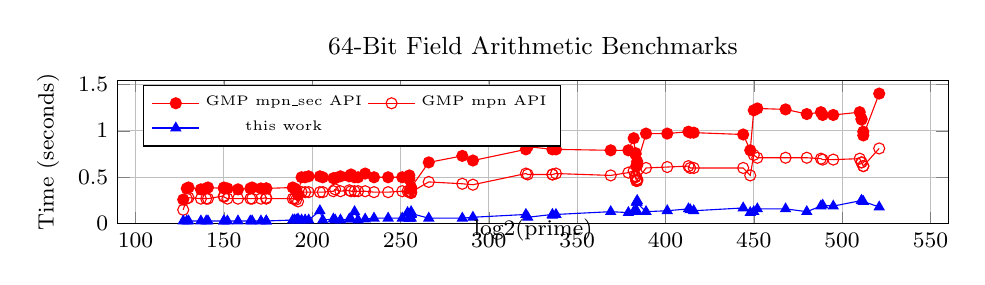
\begin{tikzpicture}
 	\begin{axis}[
 		height=3.4cm,
 		title style={font=\small},
 		title=64-Bit Field Arithmetic Benchmarks,
 		width=\textwidth,
 		legend pos= north west,
% 		xtick distance=64,
 		legend style={font=\tiny},
 		label style={font=\footnotesize},
 		xlabel style={at={(0.5,0.1)}, anchor=north},
 		legend columns=2,
 		tick label style={font=\footnotesize},
 		grid=major,
 		ymin=0,
         xmin=90,
         xmax=560,
 		xlabel=log2(prime),
 		ylabel=Time (seconds)]
		\addplot[color=red,mark=*,mark size=2pt] coordinates {
			(127.0, 0.26)
			(129.0, 0.38)
			(130.0, 0.39)
			(137.0, 0.37)
			(140.0, 0.38)
			(141.0, 0.39)
			(150.0, 0.38)
			(150.0, 0.39)
			(152.0, 0.38)
			(158.0, 0.37)
			(165.0, 0.38)
			(166.0, 0.39)
			(171.0, 0.38)
			(174.0, 0.38)
			(174.0, 0.38)
			(189.0, 0.39)
			(190.0, 0.38)
			(191.0, 0.36)
			(192.0, 0.31)
			(194.0, 0.5)
			(196.0, 0.5)
			(198.0, 0.51)
			(204.37503943134692, 0.51)
			(206.0, 0.5)
			(212.0, 0.49)
			(213.0, 0.49)
			(216.0, 0.51)
			(221.0, 0.51)
			(222.0, 0.53)
			(224.0, 0.5)
			(226.0, 0.5)
			(230.0, 0.54)
			(235.0, 0.5)
			(243.0, 0.5)
			(251.0, 0.5)
			(253.98877343250717, 0.5)
			(255.0, 0.48)
			(255.0, 0.52)
			(256.0, 0.38)
			(255.99999999966408, 0.38)
			(256.0, 0.38)
			(256.0, 0.37)
			(255.9980614856364, 0.39)
			(266.0, 0.66)
			(285.0, 0.73)
			(291.0, 0.68)
			(321.0, 0.8)
			(322.0, 0.83)
			(336.0, 0.8)
			(336.0, 0.86)
			(338.0, 0.8)
			(369.0, 0.79)
			(379.0, 0.79)
			(382.0, 0.92)
			(383.0, 0.75)
			(383.0, 0.75)
			(383.0, 0.76)
			(384.0, 0.64)
			(384.0, 0.67)
			(383.9998899269044, 0.63)
			(383.467605550083, 0.62)
			(389.0, 0.97)
			(401.0, 0.97)
			(413.0, 0.99)
			(414.0, 0.98)
			(416.0, 0.98)
			(444.0, 0.96)
			(448.0, 0.79)
			(450.0, 1.22)
			(452.0, 1.24)
			(468.0, 1.23)
			(480.0, 1.18)
			(488.0, 1.2)
			(489.0, 1.17)
			(495.0, 1.17)
			(509.97423531735535, 1.2)
			(511.0, 1.13)
			(511.0, 1.12)
			(511.9891505409899, 0.99)
			(512.0, 0.95)
			(521.0, 1.4)
		};
		\addlegendentry{GMP mpn\_sec API}

		\addplot[color=red,mark=o,mark size=2pt] coordinates {
			(127.0, 0.15)
			(129.0, 0.27)
			(130.0, 0.28)
			(137.0, 0.27)
			(140.0, 0.27)
			(141.0, 0.27)
			(150.0, 0.3)
			(150.0, 0.29)
			(152.0, 0.27)
			(158.0, 0.27)
			(165.0, 0.27)
			(166.0, 0.27)
			(171.0, 0.27)
			(174.0, 0.28)
			(174.0, 0.27)
			(189.0, 0.27)
			(190.0, 0.27)
			(191.0, 0.26)
			(192.0, 0.24)
			(194.0, 0.34)
			(196.0, 0.34)
			(198.0, 0.34)
			(204.37503943134692, 0.34)
			(206.0, 0.34)
			(212.0, 0.35)
			(213.0, 0.37)
			(216.0, 0.35)
			(221.0, 0.36)
			(222.0, 0.35)
			(224.0, 0.35)
			(226.0, 0.35)
			(230.0, 0.35)
			(235.0, 0.34)
			(243.0, 0.34)
			(251.0, 0.35)
			(253.98877343250717, 0.35)
			(255.0, 0.35)
			(255.0, 0.34)
			(256.0, 0.34)
			(255.99999999966408, 0.33)
			(256.0, 0.34)
			(256.0, 0.34)
			(255.9980614856364, 0.34)
			(266.0, 0.45)
			(285.0, 0.43)
			(291.0, 0.42)
			(321.0, 0.54)
			(322.0, 0.53)
			(336.0, 0.53)
			(336.0, 0.53)
			(338.0, 0.54)
			(369.0, 0.52)
			(379.0, 0.55)
			(382.0, 0.57)
			(383.0, 0.5)
			(383.0, 0.51)
			(383.0, 0.51)
			(384.0, 0.47)
			(384.0, 0.48)
			(383.9998899269044, 0.46)
			(383.467605550083, 0.46)
			(389.0, 0.6)
			(401.0, 0.61)
			(413.0, 0.62)
			(414.0, 0.6)
			(416.0, 0.6)
			(444.0, 0.6)
			(448.0, 0.52)
			(450.0, 0.74)
			(452.0, 0.71)
			(468.0, 0.71)
			(480.0, 0.71)
			(488.0, 0.7)
			(489.0, 0.69)
			(495.0, 0.69)
			(509.97423531735535, 0.7)
			(511.0, 0.66)
			(511.0, 0.66)
			(511.9891505409899, 0.62)
			(512.0, 0.62)
			(521.0, 0.81)
		};
		\addlegendentry{GMP mpn API}

		\addplot[color=blue,mark=triangle*,mark size=2pt] coordinates {
			(127.0, 0.03)
			(129.0, 0.03)
			(130.0, 0.03)
			(137.0, 0.03)
			(140.0, 0.03)
			(141.0, 0.03)
			(150.0, 0.03)
			(150.0, 0.03)
			(152.0, 0.03)
			(158.0, 0.03)
			(165.0, 0.03)
			(166.0, 0.03)
			(171.0, 0.03)
			(174.0, 0.03)
			(174.0, 0.03)
			(189.0, 0.04)
			(190.0, 0.04)
			(191.0, 0.04)
			(192.0, 0.05)
			(194.0, 0.04)
			(196.0, 0.04)
			(198.0, 0.04)
			(204.37503943134692, 0.14)
			(206.0, 0.04)
			(212.0, 0.05)
			(213.0, 0.04)
			(216.0, 0.04)
			(221.0, 0.05)
			(222.0, 0.05)
			(224.0, 0.13)
			(226.0, 0.04)
			(230.0, 0.05)
			(235.0, 0.06)
			(243.0, 0.06)
			(251.0, 0.06)
			(253.98877343250717, 0.12)
			(255.0, 0.06)
			(255.0, 0.06)
			(256.0, 0.06)
			(255.99999999966408, 0.11)
			(256.0, 0.1)
			(256.0, 0.13)
			(255.9980614856364, 0.11)
			(266.0, 0.06)
			(285.0, 0.06)
			(291.0, 0.07)
			(321.0, 0.1)
			(322.0, 0.07)
			(336.0, 0.1)
			(336.0, 0.09)
			(338.0, 0.1)
			(369.0, 0.13)
			(379.0, 0.12)
			(382.0, 0.13)
			(383.0, 0.13)
			(383.0, 0.13)
			(383.0, 0.13)
			(384.0, 0.25)
			(384.0, 0.13)
			(383.9998899269044, 0.23)
			(383.467605550083, 0.23)
			(389.0, 0.13)
			(401.0, 0.14)
			(413.0, 0.16)
			(414.0, 0.15)
			(416.0, 0.14)
			(444.0, 0.17)
			(448.0, 0.12)
			(450.0, 0.13)
			(452.0, 0.16)
			(468.0, 0.16)
			(480.0, 0.13)
			(488.0, 0.19)
			(489.0, 0.2)
			(495.0, 0.19)
			(511.0, 0.25)
			(511.0, 0.25)
			(512.0, 0.24)
			(521.0, 0.18)
		};
		\addlegendentry{this work}

	\end{axis}
\end{tikzpicture}
 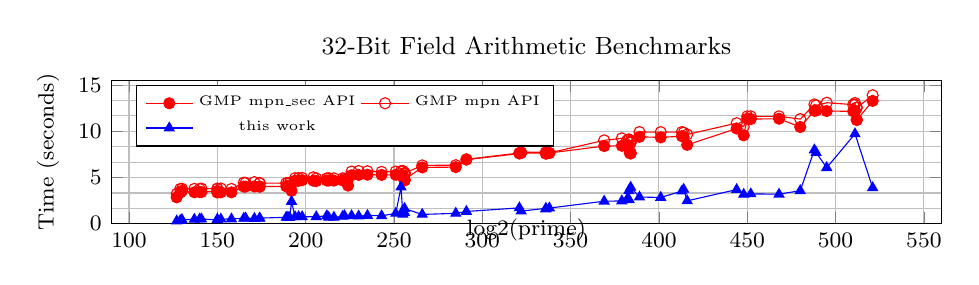
\begin{tikzpicture}
 \begin{axis}[
 ymin=0,
 ymax=15.5,
 xmin=90,
 xmax=560,
 ticks=none,
 height=3.4cm,
 width=\textwidth,
 ytick={0,1.67,3.33,5,...,15},
 %label style={font=\footnotesize},
 %xlabel style={at={(0.5,0.1)}, anchor=north},
 %tick label style={font=\footnotesize},
 grid=major,
 ]
 \end{axis}
 	\begin{axis}[
        height=3.4cm,
 		title style={font=\small},
 		title=32-Bit Field Arithmetic Benchmarks,
 		width=\textwidth,
 		legend pos= north west,
% 		xtick distance=64,
 		legend style={font=\tiny},
 		label style={font=\footnotesize},
 		xlabel style={at={(0.5,0.1)}, anchor=north},
 		legend columns=2,
 		tick label style={font=\footnotesize},
 		grid=major,
 		ymin=0,
        ymax=15.5,
        xmin=90,
        xmax=560,
 		xlabel=log2(prime),
 		ylabel=Time (seconds)]
		\addplot[color=red,mark=*,mark size=2pt] coordinates {
			(127.0, 2.86)
			(129.0, 3.38)
			(130.0, 3.56)
			(137.0, 3.41)
			(140.0, 3.43)
			(141.0, 3.43)
			(150.0, 3.56)
			(150.0, 3.38)
			(152.0, 3.4)
			(158.0, 3.4)
			(165.0, 4.02)
			(166.0, 4.02)
			(171.0, 4.04)
			(174.0, 4.03)
			(174.0, 4.02)
			(189.0, 4.05)
			(190.0, 4.1)
			(191.0, 4.03)
			(192.0, 3.56)
			(194.0, 4.66)
			(196.0, 4.64)
			(198.0, 4.72)
			(204.37503943134692, 4.66)
			(206.0, 4.62)
			(212.0, 4.68)
			(213.0, 4.68)
			(216.0, 4.67)
			(221.0, 4.68)
			(222.0, 4.72)
			(224.0, 4.13)
			(226.0, 5.25)
			(230.0, 5.29)
			(235.0, 5.31)
			(243.0, 5.29)
			(251.0, 5.3)
			(253.98877343250717, 5.26)
			(255.0, 5.25)
			(255.0, 5.27)
			(256.0, 4.71)
			(255.99999999966408, 4.7)
			(256.0, 4.72)
			(256.0, 4.77)
			(255.9980614856364, 4.78)
			(266.0, 6.1)
			(285.0, 6.13)
			(291.0, 6.94)
			(321.0, 7.6)
			(322.0, 7.66)
			(336.0, 7.64)
			(336.0, 7.58)
			(338.0, 7.66)
			(369.0, 8.41)
			(379.0, 8.44)
			(382.0, 8.41)
			(383.0, 8.44)
			(383.0, 8.47)
			(383.0, 8.45)
			(384.0, 7.62)
			(384.0, 7.62)
			(383.9998899269044, 7.64)
			(383.467605550083, 7.66)
			(389.0, 9.41)
			(401.0, 9.35)
			(413.0, 9.48)
			(414.0, 9.4)
			(416.0, 8.54)
			(444.0, 10.31)
			(448.0, 9.57)
			(450.0, 11.37)
			(452.0, 11.33)
			(468.0, 11.37)
			(480.0, 10.47)
			(488.0, 12.23)
			(489.0, 12.26)
			(495.0, 12.2)
			(509.97423531735535, 12.17)
			(511.0, 12.21)
			(511.0, 12.23)
			(511.9891505409899, 11.26)
			(512.0, 11.23)
			(521.0, 13.3)
		};
		\addlegendentry{GMP mpn\_sec API}

		\addplot[color=red,mark=o,mark size=2pt] coordinates {
			(127.0, 3.23)
			(129.0, 3.77)
			(130.0, 3.79)
			(137.0, 3.78)
			(140.0, 3.77)
			(141.0, 3.81)
			(150.0, 3.79)
			(150.0, 3.8)
			(152.0, 3.82)
			(158.0, 3.77)
			(165.0, 4.45)
			(166.0, 4.43)
			(171.0, 4.51)
			(174.0, 4.39)
			(174.0, 4.4)
			(189.0, 4.4)
			(190.0, 4.42)
			(191.0, 4.4)
			(192.0, 4.23)
			(194.0, 4.94)
			(196.0, 4.94)
			(198.0, 4.97)
			(204.37503943134692, 5.03)
			(206.0, 4.91)
			(212.0, 4.91)
			(213.0, 4.94)
			(216.0, 4.92)
			(221.0, 4.92)
			(222.0, 4.87)
			(224.0, 4.85)
			(226.0, 5.65)
			(230.0, 5.71)
			(235.0, 5.69)
			(243.0, 5.62)
			(251.0, 5.65)
			(253.98877343250717, 5.7)
			(255.0, 5.7)
			(255.0, 5.71)
			(256.0, 5.49)
			(255.99999999966408, 5.46)
			(256.0, 5.45)
			(256.0, 5.48)
			(255.9980614856364, 5.46)
			(266.0, 6.32)
			(285.0, 6.34)
			(291.0, 6.98)
			(321.0, 7.66)
			(322.0, 7.74)
			(336.0, 7.74)
			(336.0, 7.69)
			(338.0, 7.67)
			(369.0, 9.03)
			(379.0, 9.25)
			(382.0, 9.04)
			(383.0, 9.11)
			(383.0, 9.13)
			(383.0, 9.11)
			(384.0, 8.8)
			(384.0, 8.82)
			(383.9998899269044, 8.94)
			(383.467605550083, 8.84)
			(389.0, 9.93)
			(401.0, 9.92)
			(413.0, 9.93)
			(414.0, 9.86)
			(416.0, 9.67)
			(444.0, 10.89)
			(448.0, 10.51)
			(450.0, 11.63)
			(452.0, 11.63)
			(468.0, 11.63)
			(480.0, 11.33)
			(488.0, 12.92)
			(489.0, 12.81)
			(495.0, 13.1)
			(509.97423531735535, 12.9)
			(511.0, 13.07)
			(511.0, 12.9)
			(511.9891505409899, 12.58)
			(512.0, 12.55)
			(521.0, 13.91)
		};
		\addlegendentry{GMP mpn API}

		\addplot[color=blue,mark=triangle*,mark size=2pt] coordinates {
			(127.0, 0.3)
			(129.0, 0.35)
			(130.0, 0.44)
			(137.0, 0.48)
			(140.0, 0.51)
			(141.0, 0.51)
			(150.0, 0.42)
			(150.0, 0.49)
			(152.0, 0.5)
			(158.0, 0.52)
			(165.0, 0.59)
			(166.0, 0.61)
			(171.0, 0.57)
			(174.0, 0.58)
			(174.0, 0.61)
			(189.0, 0.7)
			(190.0, 0.71)
			(191.0, 0.66)
			(192.0, 2.41)
			(194.0, 0.75)
			(196.0, 0.77)
			(198.0, 0.76)
			(206.0, 0.76)
			(212.0, 0.86)
			(213.0, 0.7)
			(216.0, 0.7)
			(221.0, 0.8)
			(222.0, 0.87)
			(226.0, 0.87)
			(230.0, 0.83)
			(235.0, 0.9)
			(243.0, 0.86)
			(251.0, 1.12)
			(253.98877343250717, 3.97)
			(255.0, 1.01)
			(255.0, 1.43)
			(256.0, 1.2)
			(256.0, 1.65)
			(266.0, 1.01)
			(285.0, 1.13)
			(291.0, 1.33)
			(321.0, 1.72)
			(322.0, 1.37)
			(336.0, 1.67)
			(336.0, 1.59)
			(338.0, 1.7)
			(369.0, 2.44)
			(379.0, 2.47)
			(382.0, 2.66)
			(383.0, 2.63)
			(383.0, 2.6)
			(383.0, 3.58)
			(384.0, 3.95)
			(389.0, 2.89)
			(401.0, 2.85)
			(413.0, 3.53)
			(414.0, 3.72)
			(416.0, 2.48)
			(444.0, 3.7)
			(448.0, 3.18)
			(452.0, 3.23)
			(468.0, 3.2)
			(480.0, 3.58)
			(488.0, 7.99)
			(489.0, 7.7)
			(495.0, 6.07)
			(511.0, 9.73)
			(521.0, 3.9)
		};
		\addlegendentry{this work}

	\end{axis}
\end{tikzpicture}
\caption{\label{graphs}Performance comparison of our generated C code vs. handwritten using \texttt{libgmp}}
\end{figure*}

Saturated arithmetic is a known weak point of current compilers, resulting in implementors either opting for alternative arithmetic strategies or switching to assembly language.
Our programs are not immune to these issues: when we first ran our P-256 code, it produced incorrect output because \texttt{gcc} 7.1.1 had generated incorrect code%
\footnote{\url{https://gcc.gnu.org/bugzilla/show_bug.cgi?id=81300}, \url{https://gcc.gnu.org/bugzilla/show_bug.cgi?id=81294}}%
; \texttt{clang} 4.0 exited with a mere segmentation fault.%
\footnote{\url{https://bugs.llvm.org/show_bug.cgi?id=24943}}
Even in later compiler versions where these issues have stopped appearing, the code generated for saturated arithmetic varies a lot between compilers and is obviously suboptimal:
for example, there are ample redundant moves of carry flags, perhaps because the compilers do not consider flag registers during register allocation.
The same pattern is also present for X25519, although less pronounced: the two fastest assembly implementations listed earlier use a 4-limb saturated representation, but the speedup over 5-limb unsaturated assembly is smaller than the slowdown incurred in C code due to heavy use of carry flags.
Furthermore, expressing the same computation using intrinsics such as \verb|_mulx_u64| (variant A in the table) or using \texttt{uint128} and a bit shift (variant B) can produce a large performance difference, in different directions on different compilers.
% As arithmetic operations in our C source line up very closely with those in the \texttt{nistz256} assembly code, and as the difference between \texttt{icc} and \texttt{gcc} is bigger than the difference between our code and the fastest assembly code, we attribute most of the performance difference to low-level compilation.

The BoringSSL team had a positive enough experience with adopting our framework for Curve25519 that they decided to use our generated code to replace their P-256 implementation as well.
First, they replaced their handwritten 64-bit C implementation.
Second, while they had never bothered to write a specialized 32-bit P-256 implementation before, they also generated one with our framework.
\texttt{nistz256} remains as an option for use in server contexts where performance is critical and where patches can be applied quickly when new bugs are found.
The latter is not a purely theoretical concern -- Appendix \ref{bugsapp} contains an incomplete list of issues discovered in previous \texttt{nistz256} versions.

The two curves thus generated with our framework for BoringSSL together account for over 99\% of ECDH connections.
Chrome version 65 is the first release to use our P-256 code.

% https://boringssl-review.googlesource.com/c/boringssl/+/23244

% maybe write a section answering openssl mailing lists skepticism about
% low-level compilers, "what to do about the compiler?", basically saying it is
% critical infrastructure no matter what?

\subsection{Benchmarking All the Primes}\label{instantiate}

Even though the primes supported by the modular-reduction algorithms we implemented vastly outnumber those actually used for cryptography, we could not resist the temptation to do a breadth-oriented benchmark for plausible cryptographic parameters.
The only other implementation of constant-time modular arithmetic for arbitrary modulus sizes we found is the \verb|mpn_sec| section of the GNU Multiple Precision Arithmetic Library\footnote{\url{https://gmplib.org/}}.
We also include the non-constant-time \texttt{mpn} interface for comparison.
The list of primes to test was generated by scraping the archives of the ECC discussion list \texttt{curves@moderncrypto.org}, finding all supported textual representations of prime numbers.

One measurement in Fig. \ref{graphs} corresponds to 1000 sequential computations of a 256-bit Montgomery ladder, aiming to simulate cryptographic use accurately while still constraining the source of performance variation to field arithmetic.
A single source file was used for all \verb|mpn_sec|-based implementations; the modulus was specified as a preprocessor macro to allow compiler optimizations to try their best to specialize GMP code.
Our arithmetic functions were instantiated using standard heuristics for picking the compile-time parameters based on the shorthand textual representation of the prime, picking a champion configuration out of all cases where correctness proof succeeds, with two unsaturated and one Montgomery-based candidates.
The 64-bit trials were run on an x86 Intel Haswell processor and 32-bit trials were run on an ARMv7-A Qualcomm Krait (LG Nexus 4).

We see a significant performance advantage for our code, even compared to the GMP version that ``cheats'' by leaking secrets through timing.
Speedups range between 1.25X and 10X.
Appendix \ref{data} includes the full details, with Tables \ref{table64} and \ref{table32} recording all experimental data points, including for an additional comparison implementation in C++.
In our current experiments, compilation of saturated arithmetic in Coq times out for a handful of larger primes.
There is no inherent reason for this slowness, but our work-in-progress reimplementation of this pipeline (Section \ref{conclusion}) is designed to be executable using the Haskell extraction feature of Coq,
aiming to sidestep such performance unpredictability conclusively.

\section{Related Work}\label{related}

% I think it might make sense to organize/split this section based on whether some project or plan goes up or down in terms of abstraction level.
% First, verification projects:

% I think verif25519 is the predominant prior work, and we should give adaquate exposure unless political reasons demand otherwise.
% From the perspective of our high-level implementations, there is very little difference between the abstraction levels of verif25519 (qhasm) and HACl-star (common subset of F* with mutable state and C).
% HACL-star specifications are much nicer, but only about halfway to ours
% HACL-star proofs are slightly nicer, but only questionably so.
% HACL-star covers more code, but the additional higher-level code it covers acts as its own specification during verification.

% The second most interesting piece of prior work is gfverif, because it is fully automatic, but it is not published and is alpha-alpha quality according to the authors.
% of course, it still requires writing all the code by hand
% gröbner basis solvers are just really good for addition and multiplication, which make up the vast majority of unsaturated implementations.
% it is unclear how it could be extended to do anything beyond unsatruated modular arithmetic

% Scala LMS and other templating systems should be mentioned here

% Our main comparison to them is that our code is actually a natural expression of the algorithm
% because of this, verification is much less painful
% because of this, genericity (to the extent supported by the algorithm) is freely available

% Separately, we might think of extending our library to deal with assembly as opposde to C.
% there are some efforts that already do pretty well on this

% Vale and Jasmin deserve the current mentions

% verifiedBignum, compcert, cakeml

% a simple success criteria for a compiler: if you take handwritten assembly that is line-by-line expressible as compiler input and translate it to the input language, the compiler should not generate code slower than that assembly. This would help our P-256 code greatly.

% supporting loops is not a todo-item, we already have proofs about loops and we don't want the current C extraction to deal with them anyway

\subsection{Verified Elliptic-Curve Cryptography}

Several past projects have produced verified ECC implementations.
We first summarize them and then give a unified comparison against our new work.

Chen et al.~\cite{verif25519} verified an assembly implementation of Curve25519, using a mix of automatic SAT solving and manual Coq proof for remaining goals.
A later project by Bernstein and Schwabe~\cite{gfverif}, described as an ``alpha test,'' explores an alternative workflow using the Sage computer-algebra system.
This line of work benefits from the chance for direct analysis of common C and assembly programs for unsaturated arithmetic, so that obviously established standards of performance can be maintained.

Vale~\cite{vale} supports compile-time metaprogramming of assembly code, with a cleaner syntax to accomplish the same tasks done via Perl scripts in OpenSSL.
There is a superficial similarity to the flexible code generation used in our own work.
However, Vale and OpenSSL use comparatively shallow metaprogramming, essentially just doing macro substitution, simple compile-time offset arithmetic, and loop unrolling.
Vale has not been used to write code parameterized on a prime modulus (and OpenSSL includes no such code).
%Vale connects to Dafny in a proof-assistant-inspired style that keeps Vale itself out of the trusted code base.
A verified static analysis checks that assembly code does not leak secrets, including through timing channels.

HACL$^*$~\cite{hacl} is a cryptographic library implemented and verified in the F$^*$ programming language, providing all the functionality needed to run TLS 1.3 with the latest primitives.
Primitives are implemented in the Low$^*$ imperative subset of F$^*$~\cite{kremlin}, which supports automatic semantics-preserving translation to C.
As a result, while taking advantage of F$^*$'s high-level features for specification, HACL$^*$ performs comparably to leading C libraries.
Additionally, abstract types are used for secret data to avoid side-channel leaks.

Jasmin~\cite{jasmin} is a low-level language that wraps assembly-style straightline code with C-style control flow.
It has a Coq-verified compiler to 64-bit x86 assembly (with other targets planned), along with support for verification of memory safety and absence of information leaks, via reductions to Dafny.
A Dafny reduction for functional-correctness proof exists but has not yet been used in a significant case study.

We compare against these past projects in a few main claims.

\emph{Advantage of our work:} \textbf{first verified high-performance implementation of P-256}.
Though this curve is the most widely used in TLS today, no prior projects had demonstrated performance-competitive versions with correctness proofs.
A predecessor system to HACL$^*$~\cite{ECCstar} verified more curves, including P-256, but in high-level F$^*$ code, incurring performance overhead above 100X.

\emph{Advantage of our work:} \textbf{code and proof reuse across algorithms and parameters}.
A more fundamental appeal of our approach is that it finally enables the high-performance-cryptography domain to benefit from pleasant software-engineering practices of abstraction and code reuse.
The code becomes easier to understand and maintain (and therefore to prove), and we also gain the ability to compile fast versions of new algorithm variants automatically, with correctness proofs.
Considering the cited past work, it is perhaps worth emphasizing how big of a shift it is to do implementation and proving at a parameterized level: as far as we are aware, no past project on high-performance verified ECC has ever \emph{verified implementations of multiple elliptic curves} or \emph{verified multiple implementations of one curve, targeted at different hardware characteristics}.
With our framework, all of those variants can be generated automatically, at low developer cost; and indeed the BoringSSL team took advantage of that flexibility.

\emph{Advantage of our work:} \textbf{small trusted code base}.
Every past project we mentioned includes either an SMT solver or a computer-algebra system in the trusted code base.
Furthermore, each past project also trusts some program-verification tool that processes program syntax and outputs symbolic proof obligations.
We trust only the standard Coq theorem prover, which has a proof-checking kernel significantly smaller than the dependencies just mentioned, and the (rather short, whiteboard-level) statements of the formal claims that we make (plus, for now, the C compiler; see below).

\emph{Disadvantage of our work:} \textbf{stopping at C rather than assembly}.
Several past projects apply to assembly code rather than C code.
As a result, they can achieve higher performance and remove the C compiler from the trusted base.
Our generated code is already rather close to assembly, differing only in the need for some register allocation and instruction scheduling.
In fact, it seems worth pointing out that every phase of our code-generation pipeline is necessary to get code \emph{low-level enough} to be accepted as input by Jasmin or Vale.
We have to admit to nontrivial frustration with popular C compilers in the crypto domain, keeping us from using them to bridge this gap with low performance cost.
We wish compiler authors would follow the maxim that, if a programmer takes handwritten assembly and translates it line-by-line to the compiler's input language, the compiler should not generate code slower than the original assembly.
Unfortunately, no popular compiler seems to obey that maxim today, so we are looking into writing our own (with correctness proof) or integrating with one of the projects mentioned above.

\emph{Disadvantage of our work:} \textbf{constant-time guarantee mechanized only for straightline code}.
Our development also includes higher-level cryptographic code that calls the primitives described here, with little innovation beyond comprehensive functional-correctness proofs.
That code is written following ``constant-time'' coding rules and thus should be free of timing side channels barring human error.
However, we do not yet do certified compilation or static analysis for timing leaks on the higher-level code.
To this end, it could be advantageous to take inspiration from, or adopt, one of the tools mentioned above.

\subsection{Other Related Work}

Performance-oriented synthesis of domain-specific code (without proofs of correctness) has previously been done using explicit templates (e.g. Template Haskell~\cite{TemplateHaskell}) and more sophisticated multistage programming (e.g. Lightweight Modular Staging (LMS)~\cite{LMS}).
More specialized frameworks along these lines include FFTW~\cite{FFTW} and Spiral~\cite{SPIRAL}.
Out of these, our strategy is most similar to the one from LMS, differing mainly in the choice of using existing (proof-generating) Coq facilities for partial evaluation and rewriting rather than implementing them ourselves.
While verified compilers (e.g., CakeML~\cite{CakeML}, CompCert~\cite{Compcert}) and translation validators~\cite{NeculaTransVal} are useful for creating soundly optimized versions of a reference program, we are not aware of any that could cope with abstraction-collapsing synthesis as done in this work or LMS.

Myreen and Curello verified a general-purpose big-integer library~\cite{verifiedBignum}.
The code uses a single uniform base system, does not include specialized modular-reduction optimizations, and does not run in constant time.
However, their verification extends down to AMD64 assembly using verified decompilation.
%The proof effort is roughly similar to ours (6227 lines of HOL).

Verification of cryptographic protocols (e.g., FCF~\cite{FCF}, CertiCrypt~\cite{CertiCrypt}) is complementary to this work: given a good formal specification of a protocol, it can be shown separately that an implementation corresponds to the protocol (as we do for elliptic-curve primitives used in TLS) and that the protocol is secure (out of scope for this paper).
The work by Beringer et al.~\cite{HMAC} is a good example of this pattern, composing a protocol-security proof, a correctness proof for its C-level implementation, and a correctness proof for the C compiler.

\section{Discussion}\label{conclusion}

We would like to remark on the aspects of elliptic-curve-cryptography implementation that made this approach work as well as it did, to aid future application in other contexts.
The most general (and perhaps the most important) takeaway is that effort put into structuring code in the most instructive manner possible pays off double during verification, enough to justify the development of new tooling to make that code run fast.
In cases where generalizing an algorithm makes its operation and invariants more apparent, we think it simply makes sense to prove correctness for the general version and use partial evaluation to derive the desired code, even if a specialized implementation has already been written.

On the other hand, we do not believe that the phase distinction between arithmetic and bounds analysis is fundamental, although it is convenient.
When viewing uniform positional representations as polynomials, this distinction corresponds to finding a bound on the degree of the polynomial using partial evaluation and finding bounds on its coefficients using certified compilation, but cryptographic implementation literature (e.g.~\cite{curve25519}) has treated degree and coefficient ranges rather similarly.
We are aware of one example that would be simpler if the high-level algorithms operated on tuples $(l, x, h)$ s.t. $l \le x \le h$ instead of arbitrary-precision integers $x$.
The BoringSSL P-256 implementation that was replaced with our code used prime-shape-specific modular reduction with negative $c_i$ and avoided limb underflow by adding the modulus to a field element before any addition where the input limb ranges did not already rule out underflow.
A certified compiler that needs to preserve the exact value of each limb cannot use this strategy, but it could be encoded in the framework so far by figuring out when to add the modulus for balance in some other way in the high-level algorithm.

The bounds-analysis pipeline described in this paper only works on straight-line code, greatly simplifying the implementation.
It is geared towards being used on the bodies of inner loops where naively picking the largest available integer type for each variable would be costly, but temporaries are numerous enough that picking sizes by hand would be tedious and error-prone.
The analysis could be generalized to loops and recursion by iterating until convergence, but it is unclear whether that is called for in any application.

While we do appreciate being able to support a number of plausibly useful elliptic curves with the same (parameterized) code and proof,
we believe that engineering benefits, especially simplicity of code and proof, make this approach worth considering even when targeting a single configuration.

We find it arbitrary and unfortunate that arithmetic algorithms need to be written in continuation-passing style.
As CPS was only necessary for using Coq's term reduction for partial evaluation, writing a certified partial evaluator would be sufficient to avoid it.
Preliminary experiments have given promising results, but we have not finalized the interface yet.
We also expect that replacing the controlled term reduction with a certified compilation pass would significantly improve the compilation time.
%\todo{say something about having to remove dependent types because we don't know how to reify them?}

We would like to shrink our trusted base by connecting to a certified compiler targeting assembly.
However, existing compilers are not smart enough at mapping the data flow between instructions onto time and space available on the hardware.
Thus another fruitful future-work area is studying those optimizations, principally combined register allocation and instruction scheduling, even independently of proof.
Alternatively, hand-optimized assembly code could be checked to implement the same machine-word-level computation as our generated code using an equality-checking engine like those found in modern SMT solvers (e.g., \cite{simplify}), allowing verification of optimizations that are out-of-reach for compilers, for example effective use of vector instructions.


\section*{Acknowledgments}

This work was supported in part by a Google Research Award and National Science Foundation grants CCF-1253229, CCF-1512611, and CCF-1521584.
We benefited greatly from a fruitful collaboration with Google involving David Benjamin, Thai Duong, Adam Langley, Dominic Rizzo, and Marius Schilder.
Robert Sloan contributed to this project as a student at MIT, before joining Google.
We thank Jason Donenfeld for teaching us how to benchmark arithmetic code with Linux kernel modules, as well as for setting up benchmarks for popular Curve25519 implementations.
For comments on drafts of the paper, we thank Daniel J. Bernstein, Tej Chajed, Istvan Chung, Karl Samuel Gruetter, Ivan Kuraj, Adam Langley, Derek Leung, Devin Neal, Rahul Sridhar, Peng Wang, Ray Wang, and Daniel Ziegler.

\balance
\bibliography{fiat-crypto}

\newpage

\appendices

\section{\label{bugsapp}Study of Bugs in Similar Crypto Code}
\begin{figure*}
  \begin{tabular}{llll}
    Reference/\emph{Category}                                                           & Specification               & Implementation              & Defect       \\
 \hline \emph{Carrying}\\ \hline
 \href{https://github.com/golang/go/issues/13515}{go\#13515}               & Modular exponentiation      & \texttt{uintptr}-sized Montgomery form, Go & carry handling\\
 \href{https://tweetnacl.cr.yp.to/tweetnacl-20131229.pdf}{\cite[p. 2]{TweetNaCl}\textsuperscript{\ref{tweetnacl-correction}}} & F25519 mul, square          & \texttt{ed25519-amd64-64-24k} & carry handling\\
 \href{https://github.com/openssl/openssl/commit/29851264f11ccc70c6c0140d7e3d8d93ef5c9b11}{openssl\#ef5c9b11} & Modular exponentiation & 64-bit Montgomery form, AMD64 & carry handling\\
 \href{https://git.openssl.org/gitweb/?p=openssl.git;a=commitdiff;h=4b8736a22e758c371bc2f8b3534dc0c274acf42c;ds=sidebyside}{openssl\#74acf42c} & Poly1305 & multiple implementations & carry handling \\
 \href{https://git.lysator.liu.se/nettle/nettle/commit/c71d2c9d20eeebb985e3872e4550137209e3ce4d}{nettle\#09e3ce4d} & secp-256r1 modular reduction & & carry handling\\
 \href{https://www.openssl.org/news/secadv/20170126.txt}{CVE-2017-3732} & $x^2 \bmod m$ & Montgomery form, AMD64 assembly & \href{https://boringssl.googlesource.com/boringssl/+/d103616db14ca9587f074efaf9f09a48b8ca80cb%5E%21/}{carry, exploitable}\\
 \href{https://rt.openssl.org/Ticket/Display.html?id=1593&user=guest&pass=guest}{openssl\#1593} & P384 modular reduction & & \href{https://eprint.iacr.org/2011/633.pdf}{carry, exploitable}\\
    \href{https://web.archive.org/web/20160305001036/http://blog.skylable.com/2014/05/tweetnacl-carrybit-bug/}{tweetnacl-U32} & irrelevant & bit-twiddly C & assumed 32-bit \texttt{long}\\
    \hline \emph{Canonicalization} \\ \hline
 \href{https://github.com/agl/curve25519-donna/commit/2647eeba59fb628914c79ce691df794a8edc799f}{donna\#8edc799f} & GF($2^{255}-19$) internal to wire &  32-bit pseudo-Mersenne, C & non-canonical\\
 \href{https://git.openssl.org/gitweb/?p=openssl.git;a=commitdiff;h=b62b2454fadfccaf5e055a1810d72174c2633b8f;ds=sidebyside}{openssl\#c2633b8f} & a + b mod p256 &  Montgomery form, AMD64 assembly & \href{https://mta.openssl.org/pipermail/openssl-dev/2016-August/008179.html}{non-canonical}\\
 \href{http://seb.dbzteam.org/blog/2014/04/28/tweetnacl_arithmetic_bug.html}{tweetnacl-m15} & GF($2^{255}-19$) freeze & bit-twiddly C & bounds? typo?\\
    \hline \emph{Misc. number system} \\ \hline
 \href{https://rt.openssl.org/Ticket/Display.html?id=3607}{openssl\#3607}  & P-256 field element squaring & 64-bit Montgomery form, AMD64 & limb overflow\\
 \href{https://git.openssl.org/gitweb/?p=openssl.git;a=commitdiff;h=dc3c5067cd90f3f2159e5d53c57b92730c687d7e;ds=sidebyside}{openssl\#0c687d7e} & Poly1305 & 32-bit pseudo-Mersenne, x86 and ARM & bad truncation\\
 \href{https://github.com/openssl/openssl/commit/a7a44ba55cb4f884c6bc9ceac90072dea38e66d0}{CVE-2014-3570} & Bignum squaring & asm &  limb overflow\\
 \href{https://github.com/golang/crypto/commit/84e98f45760e87786b7f24603b8166a6fa09811d}{go\#fa09811d} & poly1305 reduction & AMD64 asm, missing subtraction of 3 & found quickly\\
 \href{https://git.openssl.org/gitweb/?p=openssl.git;a=commitdiff;h=bbe9769ba66ab2512678a87b0d9b266ba970db05;ds=sidebyside}{openssl\#a970db05} & Poly1305 &  Lazy reduction in x86 asm & lost bit 59\\
 \href{https://git.openssl.org/gitweb/?p=openssl.git;a=commitdiff;h=1ea8ae5090f557fea2e5b4d5758b10566825d74b;ds=sidebyside}{openssl\#6825d74b} & Poly1305 & AVX2 addition and reduction & bounds?\\
 \href{https://github.com/bitcoin-core/secp256k1/commit/5de4c5dffd22aa4510a5c97d0ad4a9c2eed71d85}{bitcoin\#eed71d85} & ECDSA-secp256k1 x*B & mixed addition Jacobian+Affine & missing case\\
    \hline \emph{Elliptic Curves} \\ \hline
 \href{https://ed25519.cr.yp.to/python/ed25519.py}{ed25519.py} & Ed25519 & accepts signatures other impls reject & missing $h \bmod l$\\
 \href{http://hg.openjdk.java.net/jdk8u/jdk8u/jdk/rev/d99101781d7e}{openjdk\#01781d7e} & EC scalarmult & mixed addition Jacobian+Affine & \href{https://twitter.com/asanso/status/887691580018176000}{missing case}\\
 \href{https://blogs.adobe.com/security/2017/03/critical-vulnerability-uncovered-in-json-encryption.html}{jose-adobe} & ECDH-ES & 5 different libraries affected & not on curve\\
 \href{http://euklid.org/pdf/ECC_Invalid_Curve.pdf}{invalid-curve} & NIST ECDH & irrelevant & not on curve\\
 \href{https://github.com/google/end-to-end/issues/340}{end-to-end\#340} & Curve25519 library & twisted Edwards coordinates & $(0, 1) = \infty$\\
 \href{https://git.openssl.org/gitweb/?p=openssl.git;a=commitdiff;h=e3057a57caf4274ea1fb074518e4714059dfcabf;ds=sidebyside}{openssl\#59dfcabf} & Weier. affine \texttt{<->} Jacobian &  Montgomery form, AMD64 and C & $\infty$ confusion\\
    \hline \emph{Crypto Primitives} \\ \hline
 \href{http://www.dest-unreach.org/socat/contrib/socat-secadv7.html}{socat\#7} & DH in Z*p & irrelevant & non-prime $p$\\
 \href{https://web.archive.org/web/20071010042708/http://www.imc.org/ietf-openpgp/mail-archive/msg14307.html}{CVE-2006-4339} & RSA-PKCS-1 sig. verification & irrelevant & padding check\\
 \href{https://getmonero.org/2017/05/17/disclosure-of-a-major-bug-in-cryptonote-based-currencies.html}{CryptoNote}
    & Anti-double-spending tag &  additive curve25519 curve point & missed order$(P) \neq l$\\
  \end{tabular}
  \caption{Survey of bugs in algebra-based cryptography implementations}\label{bugs}
\end{figure*}

Highly optimized handwritten cryptographic arithmetic implementations have an uninspiring history of serious bugs, even when written and audited by respected experts.
To get a sense of the details, we surveyed project bug trackers and other Internet sources, stopping after finding 26 bugs (each hyperlinked to its bug report) in implementation of nontrivial cryptography-specific optimizations.
Fig. \ref{bugs} summarizes our findings, in terms of 5 emergent categories.
The first three categories have to do with representing large integers using multiple machine-word-sized integers, with custom positional number systems.
Carrying is fairly analogous to the same concept in grade-school arithmetic, and canonicalization is a part of converting back from a custom representation into a standard one.
Elliptic curve formulas are part of high-level algebraic optimizations, above the level of operations on single large integers.
Crypto primitives bring it all together to provide functionality like digital signatures.

Here is a sampling of root causes behind these bugs.
\begin{itemize}
\item Mechanical errors:
One of the two bugs uncovered in OpenSSL issue 3607 was summarized by its author as ``Got math wrong :-('', which we think refers to a pencil-and-paper execution of numerical range analysis.
    The discussion was concluded when the patched version was found to be ``good for \textasciitilde{}6B random tests'' and the reviewer saw that ``there aren't any low-hanging bugs left.''
In \texttt{ed25519-amd64-64-24k}, one of 16,184 repetitive (and handwritten) lines should have been \texttt{r2 += 0 + carry} instead of \texttt{r1 += 0 + carry} \cite[p. 2]{TweetNaCl}.
\item Confusion over intermediate specifications:
OpenSSL bug 1953 was traced back to confusion between the postconditions of exact division with remainder and an operation that produces a $q$ and $r$ s.t. $x = qm + r$ but does not guarantee that $r$ is the smallest possible.
    The probability of a random test triggering this bug was bounded to $10\cdot{}2^{-29}$~\cite{OpenSSLBignumExploit}.
\item Mathematical misconceptions:
  The
    \href{https://getmonero.org/2017/05/17/disclosure-of-a-major-bug-in-cryptonote-based-currencies.html}{CryptoNote
    doublespending bug} arose from use of an algorithm on a composite-order
    elliptic curve when it is only applicable in a prime-order group.
\end{itemize}

\section{\label{data}Full Results of Many-Primes Experiments}

Tables \ref{table64} and \ref{table32} contain the full results of our performance experiments on many primes.
Recall the basic experimental setup:
\begin{itemize}
\item Scrape all prime numbers mentioned in the archives of the ECC mailing list \texttt{curves@moderncrypto.org}.  Crucially, we record not just the numeric values of the primes but also the \emph{ways in which they are expressed} in terms of additions and subtractions of powers of 2 and small multiples thereof.
\item We run a small Python script (shorter than 300 lines) to inspect the shapes of these prime formulas, using simple heuristics to choose the parameters to our Coq library: not just a prime modulus of arithmetic but also how to divide a big integer into digits and which sequence of carry operations to perform in modular reduction.  Actually, the script generates multiple variants, by considering 64-bit vs. 32-bit hardware architectures and by considering the Montgomery and Solinas arithmetic strategies.  The main operation defined in each case is a Montgomery ladder step.
\item We run our Coq pipeline on every variant, culminating in C code pretty-printed for each one.
\item 64-bit configurations are compiled and run on an x86 Linux desktop machine, while 32-bit configurations are compiled and run on an ARM Android mobile device.  We save the running time of each variation.
\item We also compile and run fixed C and C++ implementations using \texttt{libgmp}.
\end{itemize}

The three comparison implementations are:
\begin{itemize}
\item GMP C constant-time, the best comparison with the goals of the code we generate, since running time is required to be independent of integer inputs
\item GMP C variable time, taking advantage of additional optimizations that leak input values through timing
\item GMP C++, the only one of the comparison implementations that does not include manual memory management
\end{itemize}

All three comparison programs are conventional in that they are fixed C or C++ programs, where the prime modulus is set as a preprocessor macro.
It is up to the C compiler and \texttt{libgmp} to take advantage of properties of each modulus.
The final column in each table shows how much better our specialized generation does.
We take the ratio of variable-time C GMP (the fastest GMP code) to whichever of our generated variants is faster.

Some columns in the tables contain dashes in place of numbers of seconds needed for one trial.
Those spots indicate configurations where our Coq compilation currently times out or exhausts available memory.
Considering that Coq is not designed as a platform for executing an optimizing compiler, we are pleased that we get as many successful compilations as we do!
However, we continue working on optimizations to our implementation, to push up the size of prime whose code we can compile quickly.
The timing bottleneck is generally in reification, where repeated inefficient manipulation of terms and contexts by Ltac incurs significant overhead.
The memory bottleneck generally shows up at \texttt{Qed}-time.
Note also that some configurations are expected to fail to build, for instance when applying the Solinas strategy to so-called ``Montgomery-friendly'' primes like $2^{256} - 88 \cdot 2^{240} - 1$, where implementation experts would never choose Solinas.

Among successful compilations, time ranges between tens of seconds and levels best run overnight.

% \section{\label{weighing}Weighing Our Code Base}
%
% %Lacking an established method for quantifying how difficult some piece of code is to maintain, we will resort to a mix of presenting solid (but rather uninformative) numbers and providing anecdotes about our experience developing this library.
%
% % While we started working on the first version of this library two years ago, real progress was made rather sproadically.
% % We implemented new features as we figured out how to do them nicely, making no attempt to work continuously.
% % Even so, the vast majority of the work we did has been replaced with alternatives that in hindsight seem obviously superior.
% % For these reasons, we find it rather meaningless to provide any numeric estimate of developer time -- numbers from 1 person-year to 8 person years could constructed using various thresholds for counting activity.
%
% % We also do not see our library as a feat in large-scale implementation or a collection of programming pearls.
% % Out of the 38000 lines of our code relevant to this paper, around 15000 would probably be best migrated to the Coq standard library.
% % For example, this includes numerous simple lemmas about the basic operations on natural numbers and integers along with tactic code for manipulating standard library objects.
% % Maybe a half of these were additions were created for this project, with the rest being salvaged from other projects.
% % Maybe a quarter of our code (in each file) is braindead boilerplate, working around deficencies in Coq's metaprogramming facilities.
% % To maintain compatability with tactic-based code generation, we cannot use the Coq module system for parametrization and need to import definitions from other files one-by-one, specifiying their parameters again each time.
% % Similarly, to preserve sanity while writing tactics that operate on algebraic code, we wrote a 2000-line algebraic hierarchy library that mirror's Coq's standard library in most aspects but doesn't require all uses of (for example) an operation that happens to form a ring to be marked as such ahead of time.
% % Every definition in our basesytem library is duplicated in CPS and non-CPS form, and the two are proven equivalent -- while avoiding this isn't trivial, a certified CPS-compiler for the relecant fragment of Gallina would do the trick.
% % Some of this is already improving: every time Coq developers fix a bug in the \texttt{nsatz} tactic, one of our elliptic curve proofs drops from several hundred lines to one line.
% % This list could go on; measuring this library by weight is meaningless again.
%
% We can also give a short quantitative summary of our code base, as a proxy for work required to develop and maintain it.
% Just the code for unsaturated arithmetic, described in Section \ref{basesystems}, requires 160 lines (each 80 characters or less) of code and proof, which can then trivially be used to generate all unsaturated reduction examples in this paper.
% However, trying to synthesize a chained carry operation using this code would result in exponential blow-up due to loss of sharing.
% Rewriting functions in continuation-passing style to force sharing of subexpressions (as demonstrated in Section \ref{partial}), the same library grows to around 1000 lines.
% The extensions for saturated arithmetic add 800 lines, and all proofs and code we needed to add for Montgomery reduction total 1500 lines.
% For comparison, the \texttt{amd64-51} implementation of X25519 contains 1900
% lines of assembly code (with P-256 implementations being substantially longer),
% and the translator from assembly to SMT-solver formulas used by \cite{verif25519} is 8800 lines of OCaml.
% The elliptic-curves library is rather thin: a total of 1300 lines of code for 3 curve shapes and 8 point formats, including all equivalence proofs.
% Certified-compiler-phase implementations are rather verbose and sometimes include more lines for parameters than actual code: the largest one is bounds inference (about 2500 lines code+proof), adding up to a total around 15,000 lines.
% With another 15,000 lines of utility lemmas and tactics that seem reasonable candidates to move into Coq's standard library, the total development adds up to 38,000 lines.


\pagebreak
\footnotetext{\label{tweetnacl-correction}An earlier version of this paper (prepublication) incorrectly referred to this implementation as NaCl ed25519. In fact, the bug was discovered as the code underwent NaCl's auditing process and never made it into a release.}
\ %
\clearpage
\nobalance

\bottomcaption{\label{table64}Full 64-bit benchmark data. Our code tried both Solinas and Montgomery implementations for each prime, and we test against three GMP-based implementations: one that is constant-time (gmpsec), one that is variable time (gmpvar), and GMP's C++ API. Our code is constant-time, so gmpsec is the best comparison; however, even with that constraint removed from GMP and not us, we compare favorably to gmpvar.}

\tablehead{%
  \hline
  & \multicolumn{2}{c|}{\textbf{Our Code}} & \multicolumn{3}{c|}{\textbf{GMP Code}} & \\
  \cline{2-6}
  \textbf{Prime} & \textbf{Sol.} & \textbf{Mont.} & \textbf{const time} & \textbf{var time} & \textbf{C++} & \textbf{Speed\allowbreak-up} \\ \hline}
\footnotesize
\centering
\begin{xtabular}{|l|p{0.475cm}|p{0.75cm}@{}|p{0.7cm}@{}|p{0.6cm}@{}|p{0.6cm}@{}|p{0.75cm}@{}|@{}}
	$2^{127}-1$ & 0.03 & 0.04 & 0.26 & 0.15 & 0.67 & 5.0 \\
	$2^{129}-25$ & 0.03 & 0.07 & 0.38 & 0.27 & 0.8 & 9.0 \\
	$2^{130}-5$ & 0.03 & 0.09 & 0.39 & 0.28 & 0.79 & 9.33 \\
	$2^{137}-13$ & 0.03 & 0.08 & 0.37 & 0.27 & 0.8 & 9.0 \\
	$2^{140}-27$ & 0.03 & 0.08 & 0.38 & 0.27 & 0.8 & 9.0 \\
	$2^{141}-9$ & 0.03 & 0.08 & 0.39 & 0.27 & 0.83 & 9.0 \\
	$2^{150}-3$ & 0.03 & 0.08 & 0.38 & 0.3 & 0.8 & 10.0 \\
	$2^{150}-5$ & 0.03 & 0.08 & 0.39 & 0.29 & 0.84 & 9.67 \\
	$2^{152}-17$ & 0.03 & 0.08 & 0.38 & 0.27 & 0.82 & 9.0 \\
	$2^{158}-15$ & 0.03 & 0.08 & 0.37 & 0.27 & 0.76 & 9.0 \\
	$2^{165}-25$ & 0.03 & 0.08 & 0.38 & 0.27 & 0.78 & 9.0 \\
	$2^{166}-5$ & 0.03 & 0.08 & 0.39 & 0.27 & 0.79 & 9.0 \\
	$2^{171}-19$ & 0.03 & 0.08 & 0.38 & 0.27 & 0.79 & 9.0 \\
	$2^{174}-17$ & 0.03 & 0.08 & 0.38 & 0.28 & 0.78 & 9.33 \\
	$2^{174}-3$ & 0.03 & 0.08 & 0.38 & 0.27 & 0.78 & 9.0 \\
	$2^{189}-25$ & 0.04 & 0.08 & 0.39 & 0.27 & 0.8 & 6.75 \\
	$2^{190}-11$ & 0.04 & 0.08 & 0.38 & 0.27 & 0.78 & 6.75 \\
	$2^{191}-19$ & 0.04 & 0.09 & 0.36 & 0.26 & 0.78 & 6.5 \\
	$2^{192}-2^{64}-1$ & 0.05 & 0.07 & 0.31 & 0.24 & 0.79 & 4.8 \\
	$2^{194}-33$ & 0.04 & 0.12 & 0.5 & 0.34 & 0.93 & 8.5 \\
	$2^{196}-15$ & 0.04 & 0.12 & 0.5 & 0.34 & 0.89 & 8.5 \\
	$2^{198}-17$ & 0.04 & 0.12 & 0.51 & 0.34 & 0.87 & 8.5 \\
	$2^{205}-45\cdot 2^{198}-1$ & - & 0.14 & 0.51 & 0.34 & 0.87 & 2.43 \\
	$2^{206}-5$ & 0.04 & 0.14 & 0.5 & 0.34 & 0.84 & 8.5 \\
	$2^{212}-29$ & 0.05 & 0.12 & 0.49 & 0.35 & 0.87 & 7.0 \\
	$2^{213}-3$ & 0.04 & 0.13 & 0.49 & 0.37 & 0.88 & 9.25 \\
	$2^{216}-2^{108}-1$ & 0.04 & 0.12 & 0.51 & 0.35 & 0.88 & 8.75 \\
	$2^{221}-3$ & 0.05 & 0.15 & 0.51 & 0.36 & 0.89 & 7.2 \\
	$2^{222}-117$ & 0.05 & 0.12 & 0.53 & 0.35 & 0.91 & 7.0 \\
	$2^{224}-2^{96}+1$ & - & 0.13 & 0.5 & 0.35 & 0.88 & 2.69 \\
	$2^{226}-5$ & 0.04 & 0.13 & 0.5 & 0.35 & 0.92 & 8.75 \\
	$2^{230}-27$ & 0.05 & 0.13 & 0.54 & 0.35 & 0.91 & 7.0 \\
	$2^{235}-15$ & 0.06 & 0.13 & 0.5 & 0.34 & 0.89 & 5.67 \\
	$2^{243}-9$ & 0.06 & 0.13 & 0.5 & 0.34 & 0.89 & 5.67 \\
	$2^{251}-9$ & 0.06 & 0.13 & 0.5 & 0.35 & 0.94 & 5.83 \\
	$2^{254}-127\cdot 2^{240}-1$ & - & 0.12 & 0.5 & 0.35 & 0.92 & 2.92 \\
	$2^{255}-19$ & 0.06 & 0.13 & 0.48 & 0.35 & 0.9 & 5.83 \\
	$2^{255}-765$ & 0.06 & 0.13 & 0.52 & 0.34 & 0.9 & 5.67 \\
	$2^{256}-189$ & 0.06 & 0.14 & 0.38 & 0.34 & 0.87 & 5.67 \\
	\makecell{$2^{256}-2^{224}$ \\ \quad $+2^{192}+2^{96}-1$} & - & 0.11 & 0.38 & 0.33 & 0.84 & 3.0 \\
	$2^{256}-2^{32}-977$ & 0.1 & 0.12 & 0.38 & 0.34 & 0.87 & 3.4 \\
	$2^{256}-4294968273$ & 0.14 & 0.13 & 0.37 & 0.34 & 0.86 & 2.62 \\
	$2^{256}-88\cdot 2^{240}-1$ & - & 0.11 & 0.39 & 0.34 & 0.88 & 3.09 \\
	$2^{266}-3$ & 0.06 & 0.18 & 0.66 & 0.45 & 1.13 & 7.5 \\
	$2^{285}-9$ & 0.06 & 0.18 & 0.73 & 0.43 & 0.97 & 7.17 \\
	$2^{291}-19$ & 0.07 & 0.18 & 0.68 & 0.42 & 1.0 & 6.0 \\
	$2^{321}-9$ & 0.1 & 0.26 & 0.8 & 0.54 & 1.18 & 5.4 \\
	$2^{322}-2^{161}-1$ & 0.07 & 0.27 & 0.83 & 0.53 & 1.15 & 7.57 \\
	$2^{336}-17$ & 0.1 & 0.27 & 0.8 & 0.53 & 1.11 & 5.3 \\
	$2^{336}-3$ & 0.09 & 0.27 & 0.86 & 0.53 & 1.08 & 5.89 \\
	$2^{338}-15$ & 0.1 & 0.25 & 0.8 & 0.54 & 1.06 & 5.4 \\
	$2^{369}-25$ & 0.13 & 0.26 & 0.79 & 0.52 & 1.1 & 4.0 \\
	$2^{379}-19$ & 0.12 & 0.26 & 0.79 & 0.55 & 1.07 & 4.58 \\
	$2^{382}-105$ & 0.13 & 0.25 & 0.92 & 0.57 & 1.11 & 4.38 \\
	$2^{383}-187$ & 0.13 & 0.28 & 0.75 & 0.5 & 1.05 & 3.85 \\
	$2^{383}-31$ & 0.13 & 0.26 & 0.75 & 0.51 & 1.05 & 3.92 \\
	$2^{383}-421$ & 0.13 & 0.25 & 0.76 & 0.51 & 1.06 & 3.92 \\
	\makecell{$2^{384}-2^{128}$ \\ \quad $-2^{96}+2^{32}-1$} & - & 0.25 & 0.64 & 0.47 & 0.98 & 1.88 \\
	$2^{384}-317$ & 0.13 & 0.26 & 0.67 & 0.48 & 1.0 & 3.69 \\
	$2^{384}-5\cdot 2^{368}-1$ & - & 0.23 & 0.63 & 0.46 & 0.99 & 2.0 \\
	$2^{384}-79\cdot 2^{376}-1$ & - & 0.23 & 0.62 & 0.46 & 0.99 & 2.0 \\
	$2^{389}-21$ & 0.13 & - & 0.97 & 0.6 & 1.22 & 4.62 \\
	$2^{401}-31$ & 0.14 & - & 0.97 & 0.61 & 1.17 & 4.36 \\
	$2^{413}-21$ & 0.16 & - & 0.99 & 0.62 & 1.22 & 3.88 \\
	$2^{414}-17$ & 0.15 & - & 0.98 & 0.6 & 1.21 & 4.0 \\
	$2^{416}-2^{208}-1$ & 0.14 & - & 0.98 & 0.6 & 1.16 & 4.29 \\
	$2^{444}-17$ & 0.17 & - & 0.96 & 0.6 & 1.2 & 3.53 \\
	$2^{448}-2^{224}-1$ & 0.12 & - & 0.79 & 0.52 & 1.06 & 4.33 \\
	$2^{450}-2^{225}-1$ & 0.13 & - & 1.22 & 0.74 & 1.34 & 5.69 \\
	$2^{452}-3$ & 0.16 & - & 1.24 & 0.71 & 1.32 & 4.44 \\
	$2^{468}-17$ & 0.16 & - & 1.23 & 0.71 & 1.29 & 4.44 \\
	$2^{480}-2^{240}-1$ & 0.13 & - & 1.18 & 0.71 & 1.28 & 5.46 \\
	$2^{488}-17$ & 0.19 & - & 1.2 & 0.7 & 1.28 & 3.68 \\
	$2^{489}-21$ & 0.2 & - & 1.17 & 0.69 & 1.27 & 3.45 \\
	$2^{495}-31$ & 0.19 & - & 1.17 & 0.69 & 1.3 & 3.63 \\
	$2^{510}-290\cdot 2^{496}-1$ & - & - & 1.2 & 0.7 & 1.28 & - \\
	$2^{511}-187$ & 0.25 & - & 1.13 & 0.66 & 1.21 & 2.64 \\
	$2^{511}-481$ & 0.25 & - & 1.12 & 0.66 & 1.24 & 2.64 \\
	$2^{512}-491\cdot 2^{496}-1$ & - & - & 0.99 & 0.62 & 1.15 & - \\
	$2^{512}-569$ & 0.24 & - & 0.95 & 0.62 & 1.14 & 2.58 \\
	$2^{521}-1$ & 0.18 & - & 1.4 & 0.81 & 1.44 & 4.5 \\
\hline
\end{xtabular}

\clearpage

\bottomcaption{\label{table32}Full 32-bit benchmark data. Many of the 32-bit Montgomery implementations exceeded the one-hour timeout for proofs, because 32-bit code involves approximately four times as many operations. The C++ GMP program was not benchmarked on 32-bit.}

\tablehead{%
  \hline
  & \multicolumn{2}{c|}{\textbf{Our Code}} & \multicolumn{2}{c|}{\textbf{GMP Code}} & \\
  \cline{2-5}
  \textbf{Prime} & \textbf{Sol.} & \textbf{Mont.} & \textbf{const time} & \textbf{var time} & \textbf{Speed\allowbreak-up} \\ \hline}
\footnotesize
\centering
\begin{xtabular}{|l|p{0.6cm}@{}|p{0.75cm}@{}|p{0.75cm}@{}|p{0.7cm}@{}|p{0.75cm}@{}|}
	$2^{127}-1$ & 0.3 & 1.19 & 2.86 & 3.23 & 9.53 \\
	$2^{129}-25$ & 0.35 & 1.7 & 3.38 & 3.77 & 9.66 \\
	$2^{130}-5$ & 0.44 & 1.87 & 3.56 & 3.79 & 8.09 \\
	$2^{137}-13$ & 0.48 & 2.06 & 3.41 & 3.78 & 7.1 \\
	$2^{140}-27$ & 0.51 & 1.98 & 3.43 & 3.77 & 6.73 \\
	$2^{141}-9$ & 0.51 & 2.0 & 3.43 & 3.81 & 6.73 \\
	$2^{150}-3$ & 0.42 & 2.0 & 3.56 & 3.79 & 8.48 \\
	$2^{150}-5$ & 0.49 & 1.99 & 3.38 & 3.8 & 6.9 \\
	$2^{152}-17$ & 0.5 & 1.96 & 3.4 & 3.82 & 6.8 \\
	$2^{158}-15$ & 0.52 & 2.04 & 3.4 & 3.77 & 6.54 \\
	$2^{165}-25$ & 0.59 & 2.46 & 4.02 & 4.45 & 6.81 \\
	$2^{166}-5$ & 0.61 & 2.43 & 4.02 & 4.43 & 6.59 \\
	$2^{171}-19$ & 0.57 & 2.68 & 4.04 & 4.51 & 7.09 \\
	$2^{174}-17$ & 0.58 & 2.63 & 4.03 & 4.39 & 6.95 \\
	$2^{174}-3$ & 0.61 & 2.62 & 4.02 & 4.4 & 6.59 \\
	$2^{189}-25$ & 0.7 & 2.65 & 4.05 & 4.4 & 5.79 \\
	$2^{190}-11$ & 0.71 & 2.64 & 4.1 & 4.42 & 5.77 \\
	$2^{191}-19$ & 0.66 & 2.69 & 4.03 & 4.4 & 6.11 \\
	$2^{192}-2^{64}-1$ & - & 2.41 & 3.56 & 4.23 & 1.48 \\
	$2^{194}-33$ & 0.75 & - & 4.66 & 4.94 & 6.21 \\
	$2^{196}-15$ & 0.77 & - & 4.64 & 4.94 & 6.03 \\
	$2^{198}-17$ & 0.76 & - & 4.72 & 4.97 & 6.21 \\
	$2^{205}-45\cdot 2^{198}-1$ & - & - & 4.66 & 5.03 & - \\
	$2^{206}-5$ & 0.76 & - & 4.62 & 4.91 & 6.08 \\
	$2^{212}-29$ & 0.86 & - & 4.68 & 4.91 & 5.44 \\
	$2^{213}-3$ & 0.7 & - & 4.68 & 4.94 & 6.69 \\
	$2^{216}-2^{108}-1$ & 0.7 & - & 4.67 & 4.92 & 6.67 \\
	$2^{221}-3$ & 0.8 & - & 4.68 & 4.92 & 5.85 \\
	$2^{222}-117$ & 0.87 & - & 4.72 & 4.87 & 5.43 \\
	$2^{224}-2^{96}+1$ & - & - & 4.13 & 4.85 & - \\
	$2^{226}-5$ & 0.87 & - & 5.25 & 5.65 & 6.03 \\
	$2^{230}-27$ & 0.83 & - & 5.29 & 5.71 & 6.37 \\
	$2^{235}-15$ & 0.9 & - & 5.31 & 5.69 & 5.9 \\
	$2^{243}-9$ & 0.86 & - & 5.29 & 5.62 & 6.15 \\
	$2^{251}-9$ & 1.12 & - & 5.3 & 5.65 & 4.73 \\
	$2^{254}-127\cdot 2^{240}-1$ & - & 3.97 & 5.26 & 5.7 & 1.32 \\
	$2^{255}-19$ & 1.01 & - & 5.25 & 5.7 & 5.2 \\
	$2^{255}-765$ & 1.43 & - & 5.27 & 5.71 & 3.69 \\
	$2^{256}-189$ & 1.2 & - & 4.71 & 5.49 & 3.93 \\
	$2^{256}-2^{224}+2^{192}+2^{96}-1$ & - & - & 4.7 & 5.46 & - \\
	$2^{256}-2^{32}-977$ & 1.65 & - & 4.72 & 5.45 & 2.86 \\
	$2^{256}-4294968273$ & - & - & 4.77 & 5.48 & - \\
	$2^{256}-88\cdot 2^{240}-1$ & - & - & 4.78 & 5.46 & - \\
	$2^{266}-3$ & 1.01 & - & 6.1 & 6.32 & 6.04 \\
	$2^{285}-9$ & 1.13 & - & 6.13 & 6.34 & 5.42 \\
	$2^{291}-19$ & 1.33 & - & 6.94 & 6.98 & 5.22 \\
	$2^{321}-9$ & 1.72 & - & 7.6 & 7.66 & 4.42 \\
	$2^{322}-2^{161}-1$ & 1.37 & - & 7.66 & 7.74 & 5.59 \\
	$2^{336}-17$ & 1.67 & - & 7.64 & 7.74 & 4.57 \\
	$2^{336}-3$ & 1.59 & - & 7.58 & 7.69 & 4.77 \\
	$2^{338}-15$ & 1.7 & - & 7.66 & 7.67 & 4.51 \\
	$2^{369}-25$ & 2.44 & - & 8.41 & 9.03 & 3.45 \\
	$2^{379}-19$ & 2.47 & - & 8.44 & 9.25 & 3.42 \\
	$2^{382}-105$ & 2.66 & - & 8.41 & 9.04 & 3.16 \\
	$2^{383}-187$ & 2.63 & - & 8.44 & 9.11 & 3.21 \\
	$2^{383}-31$ & 2.6 & - & 8.47 & 9.13 & 3.26 \\
	$2^{383}-421$ & 3.58 & - & 8.45 & 9.11 & 2.36 \\
	$2^{384}-2^{128}-2^{96}+2^{32}-1$ & - & - & 7.62 & 8.8 & - \\
	$2^{384}-317$ & 3.95 & - & 7.62 & 8.82 & 1.93 \\
	$2^{384}-5\cdot 2^{368}-1$ & - & - & 7.64 & 8.94 & - \\
	$2^{384}-79\cdot 2^{376}-1$ & - & - & 7.66 & 8.84 & - \\
	$2^{389}-21$ & 2.89 & - & 9.41 & 9.93 & 3.26 \\
	$2^{401}-31$ & 2.85 & - & 9.35 & 9.92 & 3.28 \\
	$2^{413}-21$ & 3.53 & - & 9.48 & 9.93 & 2.69 \\
	$2^{414}-17$ & 3.72 & - & 9.4 & 9.86 & 2.53 \\
	$2^{416}-2^{208}-1$ & 2.48 & - & 8.54 & 9.67 & 3.44 \\
	$2^{444}-17$ & 3.7 & - & 10.31 & 10.89 & 2.79 \\
	$2^{448}-2^{224}-1$ & 3.18 & - & 9.57 & 10.51 & 3.01 \\
	$2^{450}-2^{225}-1$ & - & - & 11.37 & 11.63 & - \\
	$2^{452}-3$ & 3.23 & - & 11.33 & 11.63 & 3.51 \\
	$2^{468}-17$ & 3.2 & - & 11.37 & 11.63 & 3.55 \\
	$2^{480}-2^{240}-1$ & 3.58 & - & 10.47 & 11.33 & 2.92 \\
	$2^{488}-17$ & 7.99 & - & 12.23 & 12.92 & 1.53 \\
	$2^{489}-21$ & 7.7 & - & 12.26 & 12.81 & 1.59 \\
	$2^{495}-31$ & 6.07 & - & 12.2 & 13.1 & 2.01 \\
	$2^{510}-290\cdot 2^{496}-1$ & - & - & 12.17 & 12.9 & - \\
	$2^{511}-187$ & 9.73 & - & 12.21 & 13.07 & 1.25 \\
	$2^{511}-481$ & - & - & 12.23 & 12.9 & - \\
	$2^{512}-491\cdot 2^{496}-1$ & - & - & 11.26 & 12.58 & - \\
	$2^{512}-569$ & - & - & 11.23 & 12.55 & - \\
	$2^{521}-1$ & 3.9 & - & 13.3 & 13.91 & 3.41 \\
\hline
\end{xtabular}
\end{document}
